\begin{chapterpage}{Inference for numerical data}
  \chaptertitle{Inference for numerical data}
  \label{inferenceForNumericalData}
  \label{ch_inference_for_means}
  \chaptersection{oneSampleMeansWithTDistribution}
  \chaptersection{pairedData}
  \chaptersection{theTDistributionForTheDifferenceOfTwoMeans}
\end{chapterpage}
%\chapter{Inference for means}
 % \label{ch_inference_for_means}

\renewcommand{\chapterfolder}{ch_inference_for_means}


\chapterintro{Chapter~\ref{foundationsForInference} introduced a framework for statistical inference based on confidence intervals and hypothesis tests. Chapter~\ref{inferenceForCategoricalData} summarized inference procedures for categorical data (counts and proportions), using the normal distribution and the chi-square distribution. In this chapter, we focus on inference procedures for numerical data and we encounter a new distribution. In each case, the inference ideas remain the same:
\begin{enumerate}
\setlength{\itemsep}{0mm}
\item Determine which point estimate or test statistic is useful.
\item Identify an appropriate distribution for the point estimate or test statistic.
\item Apply the ideas from Chapter~\ref{foundationsForInference} using the distribution from step~2.
\end{enumerate}
Each section in Chapter~\ref{inferenceForNumericalData} explores a new situation: a~single mean~(\ref{oneSampleMeansWithTDistribution}), a mean of differences~(\ref{pairedData}); and a difference of means~(\ref{theTDistributionForTheDifferenceOfTwoMeans}).

}
%_________________________________
\section[Inference for a mean with the $t$-distribution]{Inference for a mean with the \pmb{$t$}-distribution}
\label{oneSampleMeansWithTDistribution}%


\sectionintro{
\noindent%
In this section, we turn our attention to numerical variables and answer questions such as the following:  
\begin{itemize}
\item How well  can we estimate the mean income of people in a certain city, county, or state?
\item What is the average mercury content in various types of fish?
\item Are people's run times getting faster or slower, on average?
\item How does the sample size affect the expected error in our estimates?
\item
    When is it reasonable to model the sample mean $\bar{x}$
    using a normal distribution, and when will we need to use
    a new distribution, known as the $t$-distribution?
\end{itemize}


%%
\subsection*{Learning objectives}
\begin{enumerate}
\setlength{\itemsep}{0mm}
\item Understand the relationship between a $t$-distribution and a normal distribution, and explain why we use a $t$-distribution for inference on a mean.

\item State and verify whether or not the conditions for inference for a mean based on the $t$-distribution are met.  Understand when it is necessary to look at the distribution of the sample data.

\item Know the degrees of freedom associated with a one sample $t$-procedure.

\item Carry out a complete hypothesis test for a single mean.

\item Carry out a complete confidence interval procedure for a single mean.

\item Find the minimum sample size needed to estimate a mean with C\% confidence and a margin of error no greater than a certain value. 


\end{enumerate}
}

%subsection[Nearly normal population with known SD]{Nearly normal population with known SD}
%%
%%
\subsection[Using a normal distribution for inference when $\sigma$ is known]{Using a normal distribution for inference when \pmb{$\sigma$} is known}
\label{nearlyNormalPopWithKnownSD}

In Section~\ref{distributionofxbar} we saw that the distribution of a sample mean is normal if the population is normal or if the sample size is at least 30. In these problems, we used the population mean and population standard deviation to find a Z-score. However, in the case of inference, these values will be unknown. In rare circumstances we may know the standard deviation of a population, even though we do not know its mean. For example, in some industrial processes, the mean may be known to shift over time, while the standard deviation of the process remains the same. In these cases, we can use the normal model as the basis for our inference procedures. We use $\bar{x}$ as our point estimate for $\mu$ and the $SD$ formula for a sample mean calculated in Section~\ref{distributionofxbar}: $\sigma_{\bar{x}} =\frac{\sigma}{\sqrt{n}}$.  That leads to a confidence interval and a test statistic as follows:
\begin{align*}
\text{CI:  } \bar{x} &\ \pm \ z^{\star}\frac{\sigma}{\sqrt{n}}
&&Z = \frac{\bar{x} - \text{null value}}{\frac{\sigma}{\sqrt{n}}}
\end{align*}

What happens if we do not know the population standard deviation $\sigma$, as is usually the case?  The best we can do is use the sample standard deviation, denoted by $s$, to estimate the population standard deviation.
\begin{align*}
SE= \frac{s}{\sqrt{n}}
\end{align*}
However, when we do this we run into a problem:  when carrying out our inference procedures, we will be trying to estimate \emph{two} quantities: both the mean and the standard deviation. Looking at the $SD$ and $SE$ formulas, we can make some important observations that will give us a hint as to what will happen when we use $s$ instead of $\sigma$.
\begin{itemize}
\setlength{\itemsep}{0mm}
\item For a given population, $\sigma$ is a fixed number and does not vary.
\item $s$, the standard deviation of a sample, will vary from one sample to the next and will not be exactly equal to $\sigma$.
\item The larger the sample size $n$, the better the estimate $s$ will tend to be for $\sigma$.
\end{itemize}

For this reason, the normal model still works well when the sample size is large. For smaller sample sizes, we run into a problem: our use of $s$, which is used when computing the standard error, tends to add more variability to our test statistic. It is this extra variability that leads us to a new distribution: the \mbox{$t$-distribution}.


%%
%%
\subsection[Introducing the $t$-distribution]{Introducing the \pmb{$t$}-distribution}
\label{introducingTheTDistribution}

\index{t-distribution@$t$-distribution|(}

When we use the sample standard deviation $s$ in place of the population standard deviation $\sigma$ to standardize the sample mean, we get an entirely new distribution - one that is similar to the normal distribution, but has greater spread. This distribution is known as the $t$-distribution. A $t$-distribution, shown as a solid line in Figure~\ref{tDistCompareToNormalDist}, has a bell shape. However, its tails are thicker than the normal model's. We can see that a greater proportion of the area under the $t$-distribution is beyond 2 standard units from 0 than under the normal distribution.  These extra thick tails are exactly the correction we need to resolve the problem of a poorly estimated standard deviation.

\begin{figure}[h]
\centering
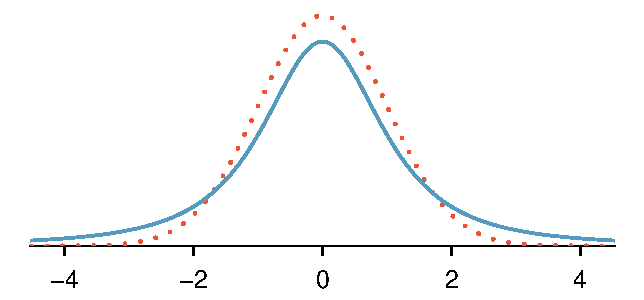
\includegraphics[width=0.58\textwidth]{ch_inference_for_means/figures/tDistCompareToNormalDist/tDistCompareToNormalDist}
\caption{Comparison of a $t$-distribution (solid line) and a normal distribution (dotted line).}
\label{tDistCompareToNormalDist}
\end{figure}

The $t$-distribution, always centered at zero, has a single parameter: degrees of freedom. The \termsub{degrees of freedom (df)}{degrees of freedom (df)!$t$-distribution} describes the precise form of the bell-shaped $t$-distribution. Several $t$-distributions are shown in Figure~\ref{tDistConvergeToNormalDist}. When there are more degrees of freedom, the $t$-distribution looks more like the standard normal distribution.

\begin{figure}[h]
\centering
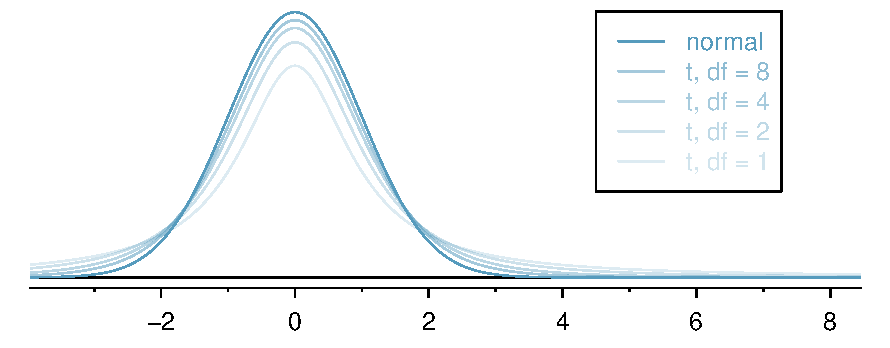
\includegraphics[width=0.83\textwidth]{ch_inference_for_means/figures/tDistConvergeToNormalDist/tDistConvergeToNormalDist}
\caption{The larger the degrees of freedom, the more closely the $t$-distribution resembles the standard normal distribution.}
\label{tDistConvergeToNormalDist}
\end{figure}

\begin{onebox}{Degrees of freedom}
The degrees of freedom describes the shape of the $t$-distribution. The larger the degrees of freedom, the more closely the distribution resembles the standard normal~distribution.\end{onebox}

When the degrees of freedom is large, about 30 or more, the $t$-distribution is nearly indistinguishable from the normal distribution. In Section~\ref{tDistSolutionToSEProblem}, we will see how degrees of freedom relates to sample size.

We will find it useful to become familiar with the $t$-distribution, because it plays a very similar role to the normal distribution during inference.  We use a \termsub{$\pmb{t}$-table}
    {t-table@$t$-table}, partially shown in Figure~\ref{tTableSample_ch_inf_means}, in place of the normal probability table when the population standard deviation is unknown, especially when the sample size is small. A~larger table is presented in Appendix~\ref{tDistributionTable}.

\begin{figure}[hht]
\centering
\begin{tabular}{r | rrr rr}
one tail & \hspace{1.5mm}  0.100 & \hspace{1.5mm} 0.050 & \hspace{1.5mm} 0.025 & \hspace{1.5mm} 0.010 & \hspace{1.5mm} 0.005  \\
\hline
{$df$} \hfill 1  &  {\normalsize  3.078} & {\normalsize  6.314} & {\normalsize 12.71} & {\normalsize 31.82} & {\normalsize 63.66}  \\
2  &  {\normalsize  1.886} & {\normalsize  2.920} & {\normalsize  4.303} & {\normalsize  6.965} & {\normalsize  9.925}  \\
3  &  {\normalsize  1.638} & {\normalsize  2.353} & {\normalsize  3.182} & {\normalsize  4.541} & {\normalsize  5.841}  \\
$\vdots$ & $\vdots$ &$\vdots$ &$\vdots$ &$\vdots$ & \\
17  &  {\normalsize  1.333} & {\normalsize  1.740} & {\normalsize  2.110} & {\normalsize  2.567} & {\normalsize  2.898}  \\
\highlightO{18}  &  \highlightO{\normalsize  1.330} & \highlightO{\normalsize  1.734} & \highlightO{\normalsize  2.101} & \highlightO{\normalsize  2.552} & \highlightO{\normalsize  2.878}  \\
19  &  {\normalsize  1.328} & {\normalsize  1.729} & {\normalsize  2.093} & {\normalsize  2.539} & {\normalsize  2.861}  \\
20  &  {\normalsize  1.325} & {\normalsize  1.725} & {\normalsize  2.086} & {\normalsize  2.528} & {\normalsize  2.845}  \\
$\vdots$ & $\vdots$ &$\vdots$ &$\vdots$ &$\vdots$ & \\
1000  &  {\normalsize  1.282} & {\normalsize  1.646} & {\normalsize  1.962} & {\normalsize  2.330} & {\normalsize  2.581}  \\
$\infty$   &  {\normalsize  1.282} & {\normalsize  1.645} & {\normalsize  1.960} & {\normalsize  2.326} & {\normalsize  2.576}   \\
\hline
Confidence level C  &  {\normalsize  80\%} & {\normalsize 90\%} & {\normalsize 95\%} & {\normalsize  98\%} & {\normalsize  99\%}  \\
\hline
\end{tabular}
\caption{An abbreviated look at the $t$-table. Each row represents a different $t$-distribution. The columns describe the cutoffs for specific tail areas. The row with $df=18$ has been \highlightO{highlighted}.}
\label{tTableSample_ch_inf_means}
\end{figure}

Each row in the $t$-table represents a $t$-distribution with different degrees of freedom. The columns correspond to tail probabilities. For instance, if we know we are working with the $t$-distribution with $df=18$, we can examine row 18, which is \highlightO{highlighted} in Figure~\ref{tTableSample_ch_inf_means}. If we want the value in this row that identifies the cutoff for an upper tail of 10\%, we can look in the column where \emph{one tail} is 0.100. This cutoff is 1.33. If we had wanted the cutoff for the lower 10\%, we would use -1.33. Just like the normal distribution, all $t$-distributions are symmetric.


\begin{examplewrap}
\begin{nexample}{What proportion of the $t$-distribution with 18 degrees of freedom falls below -2.10?}
Just like a normal probability problem, we first draw a picture as shown in Figure~\ref{tDistDF18LeftTail2Point10} and shade the area below -2.10. To find this area, we identify the appropriate row: $df=18$. Then we identify the column containing the absolute value of -2.10; it is the third column. Because we are looking for just one tail, we examine the top line of the table, which shows that a one tail area for a value in the third row corresponds to 0.025. That is, 2.5\% of the distribution falls below -2.10.
\end{nexample}
\end{examplewrap}

\begin{figure}
\centering
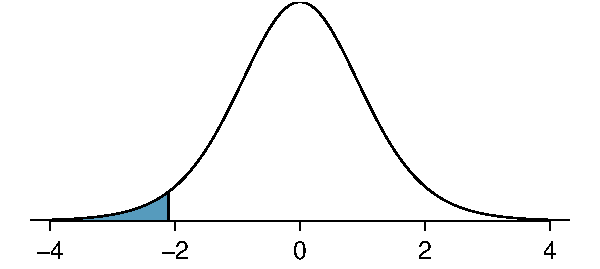
\includegraphics[width=0.53\textwidth]{ch_inference_for_means/figures/tDistDF18LeftTail2Point10/tDistDF18LeftTail2Point10}
\caption{The $t$-distribution with 18 degrees of freedom. The area below -2.10 has been shaded.}
\label{tDistDF18LeftTail2Point10}
\end{figure}


\begin{examplewrap}
\begin{nexample}{For the $t$-distribution with 18 degrees of freedom, what percent of the curve is contained between -1.330 and +1.330?}
Using row $df = 18$, we find 1.330 in the table. The area in each tail is 0.100 for a total of 0.200, which leaves 0.800 in the middle between -1.33 and +1.33. This corresponds to the 80\%, which can be found at the very bottom of that  column.  
\end{nexample}
\end{examplewrap}

\begin{examplewrap}
\begin{nexample}{For the $t$-distribution with 3 degrees of freedom, as shown in the left panel of Figure~\ref{tDistDF3_and_20}, what should the value of $t^{\star}$ be so that 95\% of the area of the curve falls between -$t^{\star}$ and +$t^{\star}$?}
We can look at the column in the $t$-table that says 95\% along the bottom row and trace it up to row $df = 3$ to find that $t^{\star} = 3.182$.
\end{nexample}
\end{examplewrap}

\begin{examplewrap}
\begin{nexample}{A $t$-distribution with 20 degrees of freedom is shown in the right panel of Figure~\ref{tDistDF3_and_20}. Estimate the proportion of the distribution falling above 1.65.}
We identify the row in the $t$-table using the degrees of freedom: $df=20$. Then we look for 1.65; it is not listed. It falls between the first and second columns. Since these values bound 1.65, their tail areas will bound the tail area corresponding to 1.65. We identify the one tail area of the first and second columns, 0.050 and 0.10, and we conclude that between 5\% and 10\% of the distribution is more than 1.65 standard deviations above the mean. If we like, we can identify the precise area using statistical software: 0.0573.
\end{nexample}
\end{examplewrap}

\begin{figure}
\centering
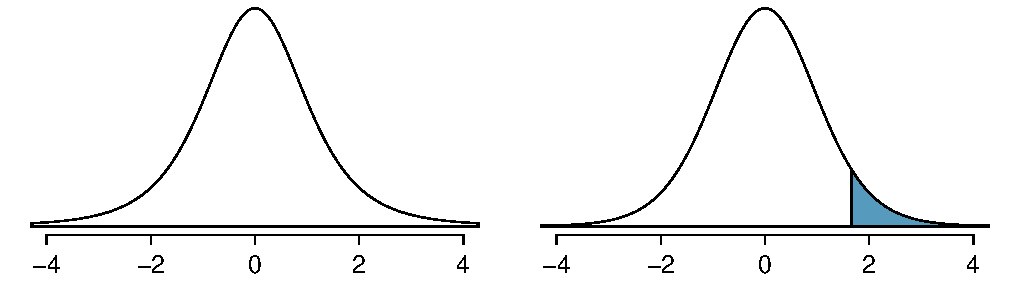
\includegraphics[width=0.93\textwidth]{ch_inference_for_means/figures/tDistDF3_and_20/tDistDF3_and_20}
\caption{Left: The $t$-distribution with 3 degrees of freedom, with the area farther than 3.182 units from 0 shaded.  Right: The $t$-distribution with 20 degrees of freedom, with the area above 1.65 shaded.}
\label{tDistDF3_and_20}
\end{figure}

When the desired degrees of freedom is not listed on the table, choose a conservative value: round the degrees of freedom down, i.e. move \emph{up} to the previous row listed. Another option is to use a calculator or statistical software to get a precise answer.


\D{\newpage}

%%
\subsection[Calculator: finding area under the $t$-distribution]{Calculator: finding area under the \pmb{$t$}-distribution}

It is possible to find areas under a $t$-distribution on a calculator.

\begin{onebox}{TI-84: Finding area under the T-curve}
Use \calcbutton{2ND} \calcbutton{VARS}, \calctext{tcdf} to find an area/proportion/probability between two $t$-scores or to the left or right of a $t$-score.\vspace{-1mm}
\begin{enumerate}
\setlength{\itemsep}{0mm}
\item Choose \calcbutton{2ND} \calcbutton{VARS} (i.e. \calctext{DISTR}).
\item Choose \calctext{6:tcdf}.
\item Enter the \calctext{lower} (left) $t$-score and the \calctext{upper} (right) $t$-score.
\vspace{-1.5mm}
  \begin{itemize}
  \setlength{\itemsep}{0mm}
  \item If finding just a lower tail area, set \calctext{lower} to \calctext{-100}.
  \item For an upper tail area, set \calctext{upper} to \calctext{100}.
\end{itemize}
\item Enter the degrees of freedom after \calctext{df:}.
\item Down arrow, choose \calctext{Paste}, and hit \calcbutton{ENTER}.\vspace{-1.5mm}
\end{enumerate}
TI-83: Do steps 1-2, then enter the lower bound, upper bound, degrees of freedom, e.g. \calctext{tcdf(2, 100, 5)}, and hit \calcbutton{ENTER}.\end{onebox}

\begin{onebox}{Casio fx-9750GII: Finding area under the T-distribution}
\begin{enumerate}
\setlength{\itemsep}{0mm}
\item Navigate to \calctext{STAT} (\calcbutton{MENU}, then hit \calcbutton{2}).
\item Select \calctext{DIST} (\calcbutton{F5}), then \calctext{t} (\calcbutton{F2}), and then \calctext{tcd} (\calcbutton{F2}).
\item If needed, set \calctext{Data} to \calctext{Variable} (\calctext{Var} option, which is \calcbutton{F2}).
\item Enter the \calctext{Lower} $t$-score and the \calctext{Upper} $t$-score. Set the degrees of freedom (\calctext{df}).\vspace{-1.5mm}
  \begin{itemize}
  \setlength{\itemsep}{0mm}
  \item If finding just a lower tail area, set \calctext{Lower} to \calctext{-100}.
  \item For an upper tail area, set \calctext{Upper} to \calctext{100}.
  %\item If finding a middle area (e.g. $Z_{lower} = 0.5$ to $Z_{upper} = 1.5$), set the \calctext{lower} and \calctext{upper} values appropriately.
  \end{itemize}
\item Hit \calctext{EXE}, which will return the area probability (\calctext{p}) along with the $t$-scores for the lower and upper bounds.
\end{enumerate}
\end{onebox}
 
\begin{exercisewrap}
\begin{nexercise}Use a calculator to find the area to the right of $t=3$ under the $t$-distribution with 35 degrees of freedom.\footnotemark
\end{nexercise}
\end{exercisewrap}
\footnotetext{Because we want to shade to the right of $t=3$, we let \calctext{lower} = 3.  There is no upper bound, so use a large value such as 100 for \calctext{upper}.  Let \calctext{df} = 35.  The area is 0.0025 or 0.25\%.}

\begin{exercisewrap}
\begin{nexercise}Without doing any calculations, will the area to the right of $Z=3$ under the standard normal curve be greater than, less than, or equal to the area to the right of $t=3$ with 35 degrees of freedom?\footnotemark
\end{nexercise}
\end{exercisewrap} 
\footnotetext{Because the $t$-distribution has greater spread and thicker tails than the normal distribution, we would expect the upper tail area to the right of $Z=3$ to be less than the upper tail area to the right of $t=3$.  One can confirm that the area to the right of $Z = 3$ is 0.0013, which is less than 0.0025.  With a smaller degrees of freedom, this difference would be even more pronounced.  Try it!}

\index{t-distribution@$t$-distribution|)}


\D{\newpage}

%%
\subsection[Checking conditions for inference on a mean using the $t$-distribution]{Checking conditions for inference on a mean using the \pmb{$t$}-distribution}
\label{tDistSolutionToSEProblem}

Using the $t$-distribution for inference on a mean requires two assumptions, namely that the observations are independent and that the theoretical sampling distribution of the sample mean $\bar{x}$ is nearly normal.  In practice, we check whether these assumptions are reasonable by verifying that certain conditions are met.  


\begin{description}
\setlength{\itemsep}{0mm}
\item[Independent.] Observations can be considered independent when the data are collected from a \emph{random process}, such as tossing a coin, or from a \emph{random sample}.    Without a random sample or process, the standard error formula would not apply, and it is unclear to what population the inference would apply.  Recall from Chapter~\ref{ch_inference_for_props} that when sampling without replacement from a finite population, the observations can be considered independent when sampling less than 10\% of the population.  
\item[Nearly normal sampling distribution.] We saw in Section~\ref{distributionofxbar} that the sampling distribution of a sample mean will be nearly normal when the sample is drawn from a nearly normal population or when the sample size is at least 30 ($n\ge 30$).     
\end{description}

What should we do when the sample size is small and we are not sure whether the population distribution is nearly normal?  In this case, the best we can do is look at the data for excessive skew.  If the data are very skewed or have obvious outliers, this suggests that the sample did not come from a nearly normal population.  However, if the data do not show obvious skew or outliers, then the idea of a nearly normal population is generally considered \emph{reasonable}, making the assumption of a nearly normal sampling distribution for $\bar{x}$ reasonable as well.

Note that by looking at a small data set, we cannot \emph{prove} that the population distribution is nearly normal.  However, the data can suggest to us whether the population distribution being nearly normal is an unreasonable assumption.  

\begin{onebox}{The normality condition with small samples}
{If the sample is small and there is strong skew or extreme outliers in the data, the population from which the sample was drawn may not be nearly normal. }
\end{onebox}

Ideally, we use a graph of the data to check for strong skew or outliers.  When the full data set is not available, summary statistics can also be used. 

As the sample size goes up, it becomes less necessary to check for skew in the data.  If the sample size is 30 or more, it is no longer necessary that the population distribution be nearly normal.  When the sample size is large, the Central Limit Theorem tells us that the sampling distribution of the sample mean will be nearly normal regardless of the distribution of the population.



%%
\subsection[One sample $t$-interval for a mean]{One sample \pmb{$t$}-interval for a mean}
\label{oneSampleTConfidenceIntervals}

Dolphins are at the top of the oceanic food chain, which causes dangerous substances such as mercury to concentrate in their organs and muscles. This is an important problem for both dolphins and other animals, like humans, who eat them.
\setlength{\captionwidth}{86mm}

\begin{figure}[h]
\centering
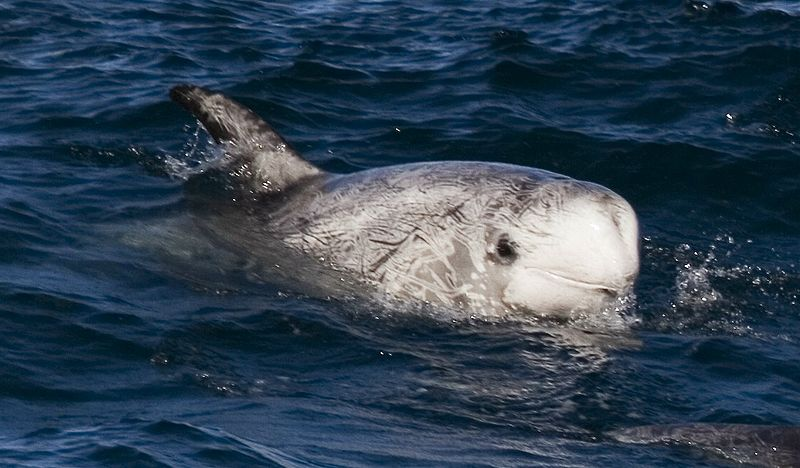
\includegraphics[width=0.7\textwidth]{ch_inference_for_means/figures/rissosDolphin/rissosDolphin.jpg}  \\
\addvspace{2mm}
\begin{minipage}{\textwidth}
   \caption[rissosDolphinPic]{A Risso's dolphin.\vspace{-1mm} \\
   -----------------------------\vspace{-2mm}\\
   {\footnotesize Photo by Mike Baird (\oiRedirect{textbook-bairdphotos_com}{www.bairdphotos.com}). \oiRedirect{textbook-CC_BY_2}{CC~BY~2.0~license}.\vspace{-10mm}}}
   \label{rissosDolphin}
\end{minipage}
\vspace{3mm}
\end{figure}
\setlength{\captionwidth}{\mycaptionwidth}

We would like to create a confidence interval to estimate the average mercury content in dolphin muscles.  We will use a sample of 19 Risso's dolphins from the Taiji area in Japan.  The data are summarized in Figure~\ref{summaryStatsOfHgInMuscleOfRissosDolphins}. 

\begin{figure}[h]
\centering
\begin{tabular}{ccc cc}
\hline
$n$ & $\bar{x}$ & $s$ & minimum & maximum \\
19   & 4.4	  & 2.3  & 1.7	       & 9.2 \\
\hline
\end{tabular}
\caption{Summary of mercury content in the muscle of 19 Risso's dolphins from the Taiji area. Measurements are in $\mu$g/wet g (micrograms of mercury per wet gram of muscle).}
\label{summaryStatsOfHgInMuscleOfRissosDolphins}
\end{figure}

Because we are estimating a mean, we would like to construct a $t$-interval, but first we must check whether the conditions for using a $t$-interval are met.  We will start by assuming that the sample of 19 Risso's dolphins constitutes a random sample.  Next, we note that the sample size is small (less than 30), and we do not know whether the distribution of mercury content for all dolphins is nearly normal.  Therefore, we must look at the data.  Since we do not have all of the data to graph, we look at the summary statistics provided in Figure~\ref{summaryStatsOfHgInMuscleOfRissosDolphins}. These summary statistics do not suggest any strong skew or outliers; all observations are within 2.5 standard deviations of the mean. Based on this evidence, we believe it is reasonable that the population distribution of mercury content in dolphins could be nearly normal.  

With both conditions met, we will construct a 95\% confidence interval.  Recall that a confidence interval has the following form:
\begin{eqnarray*}
\text{point estimate} \ \pm\  \text{critical value}\times SE\text{ of estimate}
\end{eqnarray*}
The point estimate is the sample mean and the $SE$ of the sample mean is given by $s/\sqrt{n}$.  What do we use for the critical value?  Since we are using the $t$-distribution, we use a $t$-table to find the critical value.  We denote the critical value $t^{\star}$.
\begin{itemize}
\setlength{\itemsep}{0mm}
\item For a 95\% confidence interval, we want to find the cutoff $t^{\star}$ such that 95\% of the $t$-distribution is between -$t^{\star}$ and $t^{\star}$.
\item Using the $t$-table on page~\pageref{tTableSample_ch_inf_means}, we look at the row that corresponds to the degrees of freedom and the column that corresponds to the confidence level.
\end{itemize}

\begin{onebox}{Degrees of freedom for a single sample}
If the sample has $n$ observations and we are examining a single mean, then we use the $t$-distribution with $df=n-1$ degrees of freedom.
\end{onebox}

\begin{examplewrap}
\begin{nexample}
{Calculate a 95\% confidence interval for the average mercury content in dolphin muscles based on this sample. Recall that $n=19$, $\bar{x}=4.4$ $\mu$g/wet g, and $s=2.3$ $\mu$g/wet g.  }
To find the critical value $t^{\star}$ we use the $t$-distribution with $n-1$ degrees of freedom.  The sample size is 19, so $df=19-1=18$ degrees of freedom.  Using the $t$-table with row $df=18$ and column corresponding to a 95\% confidence level, we get $t^{\star}=2.10$.  The point estimate is the sample mean $\bar{x}$ and the standard error of a sample mean is given by $\frac{s}{\sqrt{n}}$.  Now we have all the pieces we need to calculate a 95\% confidence interval for the average mercury content in dolphin muscles.  
\begin{align*}
\text{point estimate} \ &\pm\  \text{critical value} \times SE \ \text{of estimate} \\
\bar{x} \ &\pm\  t^{\star}\times \frac{s}{\sqrt{n}} \qquad df=n-1\\
4.4 \ &\pm\  2.10 \times  \frac{2.3}{\sqrt{19}} \quad df=18 \\
= &\ (3.29 \text{, } 5.51)
\end{align*}

\end{nexample}
\end{examplewrap}

\begin{examplewrap}
\begin{nexample}
{How do we interpret this 95\% confidence interval?  To what population is it applicable?}
A random sample of Risso's dolphins was taken from the Taiji area in Japan.  The mercury content in the muscles of other types of dolphins and from dolphins from other regions may vary.  Therefore, we can only make an inference to Risso's dolphins from this area.  We are 95\% confident the true average mercury content in the muscles of Risso's dolphins in the Taiji area of Japan is between 3.29 and 5.51 $\mu$g/wet gram. 

\end{nexample}
\end{examplewrap}
\index{data!dolphins and mercury|)}



\begin{onebox}{Constructing a confidence interval for a mean}
To carry out a complete confidence interval procedure to estimate a single \mbox{mean $\mu$,}
\\
\\
\inferencestep{Identify} Identify the parameter and the confidence level, C\%. \vspace{-1mm}
\begin{itemize} 
\item[] The parameter will be an unknown population mean, e.g. the true mean (or average) mercury content in Risso's dolphins.
\end{itemize}
\inferencestep{Choose} Choose the appropriate interval procedure and identify it by name.\vspace{-1mm}
\begin{itemize}
\item[] Here we choose the \term{1-sample $t$-interval}.
\end{itemize}
\inferencestep{Check} Check conditions for the sampling distribution of $\bar{x}$ to nearly normal.\vspace{-1mm}
\begin{itemize}
\setlength{\itemsep}{0mm}
\item[] 1. Data come from a random sample or random process.
\item[] 2. The sample size $n\ge 30$ or the population distribution is nearly normal.
\item[] \quad \ If the sample size is less than 30 and the population distribution is unknown, check 
\item[] \quad \ for strong skew or outliers in the data.  If neither is found, the condition that the 
\item[] \quad \ population distribution is nearly normal is considered reasonable.  
\end{itemize}
\inferencestep{Calculate} Calculate the confidence interval and record it in interval form. 
\begin{itemize}
\item[] $\text{point estimate}\ \pm\ t^{\star} \times SE\ \text{of estimate}$, \quad $df = n - 1$
\begin{itemize}
\item[] point estimate: the sample mean $\bar{x}$
\item[] $SE$ of estimate:  $\frac{s}{\sqrt{n}}$
\item[] $t^{\star}$: use a $t$-table at row $df = n-1$ and confidence level C\%
\end{itemize}
\item[] (\underline{\ \ \ \ \ }, \underline{\ \ \ \ \ })
\end{itemize}
\inferencestep{Conclude} Interpret the interval and, if applicable, draw a conclusion in context. \vspace{-1mm}
\begin{itemize}
\item[] Here, we are C\%  confident that the true \emph{mean} of [...] is between \underline{\ \ \ \ \ } and  \underline{\ \ \ \ \ }.  A conclusion depends upon whether the interval is entirely above, is entirely below, or contains the value of interest. 
\end{itemize}\end{onebox}

\begin{examplewrap}
\begin{nexample}
{The FDA's webpage provides some data on mercury content of fish.\footnotemark\, Based on a sample of 15 croaker white fish (Pacific), a sample mean and standard deviation were computed as 0.287 and 0.069 ppm (parts per million), respectively. The 15 observations ranged from 0.18 to 0.41 ppm. Construct an appropriate 95\% confidence interval for the true average mercury content of croaker white fish (Pacific). Is there evidence that the average mercury content is greater than 0.275 ppm?  Use the five step framework to organize your work.  
}
\label{croakerWhiteFishPacificExerConditions}
\begin{description}
\item[\inferencestep{Identify}] The parameter of interest is the true mean mercury content in croaker white fish (Pacific).  We want to estimate this at the 95\% confidence level.  
\item[\inferencestep{Choose}] Because the parameter to be estimated is a single mean, we will use a 1-sample $t$-interval.
\item[\inferencestep{Check}] We will assume that the sample constitutes a random sample of croaker white fish (Pacific). The sample size $n$ is small, but there are no obvious outliers; all observations are within 2 standard deviations of the mean. If there is skew, it is not too great. Therefore we think it is reasonable that the population distribution of mercury content in croaker white fish (Pacific) could be nearly normal.  
\item[\inferencestep{Calculate}]  We will calculate the interval:
\begin{align*}
\text{point estimate}\ \pm\ t^{\star} \times SE\ \text{of estimate}
\end{align*}
The point estimate is the sample mean: $\bar{x}= 0.287$\\
\\
The $SE$ of the sample mean is: $ \frac{s}{\sqrt{n}} = \frac{0.069}{\sqrt{15}}$ \\

We find $t^{\star}$ for the one sample case using the $t$-table at row $df = n -1$ and confidence level C\%.  For a 95\% confidence level and $df = 15 - 1 = 14$, $t^{\star} = 2.145$.\\

So the 95\% confidence interval is given by:
\begin{align*}
0.287 \ \pm\  &2.145\times  \frac{0.069}{\sqrt{15}}  \qquad df = 14\\
0.287 \ \pm\  &2.145\times 0.0178 \\
=(0.2&49,\ 0.325)
\end{align*}
\item[\inferencestep{Conclude}]  We are 95\% confident that the true \emph{average} mercury content of croaker white fish (Pacific) is between 0.249 and 0.325 ppm. Because the interval contains 0.275 as well as values less than 0.275, we do not have evidence that the true average mercury content is  greater than 0.275 ppm.
\end{description}
\end{nexample}
\end{examplewrap}
\footnotetext{\oiRedirect{textbook-fda_mercury_in_fish_2010}{www.fda.gov/food/foodborneillnesscontaminants/metals/ucm115644.htm}} 


\begin{examplewrap}
\begin{nexample}
{Based on the interval calculated in Example~\ref{croakerWhiteFishPacificExerConditions} above, can we say that 95\% of croaker white fish (Pacific) have mercury content between 0.249 and 0.325 ppm?}
No.  The interval estimates the \emph{average} amount of mercury with 95\% confidence.  It is not trying to capture 95\% of the values.  
\end{nexample}
\end{examplewrap}


\D{\newpage}

%%
\subsection[Calculator: the 1-sample $t$-interval]{Calculator: the 1-sample \pmb{$t$}-interval}
\label{1SampTint}

\begin{onebox}{\videohref{ti84_1_mean_CI} TI-83/84: 1-sample T-interval}
Use \calcbutton{STAT}, \calctext{TESTS}, \calctext{TInterval}.
\begin{enumerate}
\setlength{\itemsep}{0mm}
\item Choose \calcbutton{STAT}.
\item Right arrow to \calctext{TESTS}.
\item Down arrow and choose \calctext{8:TInterval}.
\item Choose \calctext{Data} if you have all the data or \calctext{Stats} if you have the mean and standard deviation.
\begin{itemize}
\item If you choose \calctext{Data}, let \calctext{List} be \calctext{L1} or the list in which you entered your data (don't forget to enter the data!) and let \calctext{Freq} be \calctext{1}.
\item If you choose \calctext{Stats}, enter the mean, $SD$, and sample size.
\end{itemize}
\item Let \calctext{C-Level} be the desired confidence level.
\item Choose \calctext{Calculate} and hit \calcbutton{ENTER}, which returns:\\
\begin{tabular}{l l}
\calctext{(\underline{\ \ },\underline{\ \ })} & the confidence interval \\
$\calctextmath{\bar{x}}$ & the sample mean \\
\calctext{Sx} & the sample $SD$ \\
\calctext{n} & the sample size
\end{tabular}
\end{enumerate}
\end{onebox}

\begin{onebox}{\videohref{casio_1_mean_inference} Casio fx-9750GII: 1-sample T-interval}
\begin{enumerate}
\setlength{\itemsep}{0mm}
\item Navigate to \calctext{STAT} (\calcbutton{MENU} button, then hit the \calcbutton{2} button or select \calctext{STAT}).
\item If necessary, enter the data into a list.
\item Choose the \calctext{INTR} option (\calcbutton{F3} button), \calctext{t} (\calcbutton{F2} button), and \calctext{1-S} (\calcbutton{F1} button).
\item Choose either the \calctext{Var} option (\calcbutton{F2}) or enter the data in using the \calctext{List} option.
\item Specify the interval details:
  \begin{itemize}
  \setlength{\itemsep}{0mm}
  \item Confidence level of interest for \calctext{C-Level}.
  \item If using the \calctext{Var} option, enter the summary statistics. If using \calctext{List}, specify the list and leave \calctext{Freq} value at \calctext{1}.
  \end{itemize}
\item Hit the \calcbutton{EXE} button, which returns \\[1mm]
\begin{tabular}{ll}
  \calctext{Left}, \calctext{Right} & ends of the confidence interval \\
  $\calctextmath{\bar{x}}$ & sample mean \\
  \calctext{sx} & sample standard deviation \\
  \calctext{n} & sample size
\end{tabular}
\end{enumerate}
\end{onebox}


\begin{exercisewrap}
\begin{nexercise}
Use a calculator to find a 95\% confidence interval for the mean mercury content in croaker white fish (Pacific).  The sample size was 15, and the sample mean and standard deviation were computed as 0.287 and 0.069 ppm (parts per million), respectively.\footnotemark
\end{nexercise}
\end{exercisewrap}
\footnotetext{Choose \calctext{TInterval} or equivalent.  We do not have all the data, so choose \calctext{Stats} on a TI or \calctext{Var} on a Casio.  Enter $\calctextmath{\bar{x}}$ and $\calctextmath{Sx}$.  Note:  $\calctextmath{Sx}$ is the sample standard deviation (\calctext{0.069}), not the $SE$.  Let $\calctext{n}=15$ and \calctext{C-Level} = 0.95.  This should give the interval $(0.249,\ 0.325)$.}


\D{\newpage}

%%
\subsection{Choosing a sample size when estimating a mean}
\label{findingASampleSizeForACertainME}

\index{margin of error|(}
In Section~\ref{moeproportion}, we looked at sample size considerations when estimating a proportion.  We take the same approach when estimating a mean.  Recall that the margin of error is measured as the distance between the point estimate and the upper or lower bound of the confidence interval.  We want to estimate a mean with a particular confidence level while putting an upper bound on the margin of error.  What is the smallest sample size that will satisfy these conditions?

For a one sample $t$-interval, the margin of error, $ME$, is given by $ME = t^{\star}\times\frac{s}{\sqrt{n}}$.  The challenge in this case is that we need to know $n$ to find $t^{\star}$.  But $n$ is precisely what we are attempting to solve for!  Fortunately, in most cases we will have a reasonable estimate for the population standard deviation and the desired $n$ will be large, so we can use $ME = z^{\star}\times\frac{\sigma}{\sqrt{n}}$, making it easier to solve for $n$.   

\begin{examplewrap}
\begin{nexample}{Blood pressure oscillates with the beating of the heart, and the systolic pressure is defined as the peak pressure when a person is at rest. The standard deviation of systolic blood pressure for people in the U.S. is about 25 mmHg (millimeters of mercury).  How large of a sample is necessary to estimate the average systolic blood pressure of people in a particular town with a margin of error no greater than 4 mmHg using a 95\% confidence level?}\label{sampleSizeComputationForSystolicBloodPressure}
 For this problem, we want to find the sample size $n$ so that the margin of error, $ME$, is less than or equal to 4 mmHg.  We start by writing the following inequality:\vspace{-1mm}
\begin{align*}
z^{\star}\times \frac{\sigma}{\sqrt{n}} \leq 4
\end{align*}
For a 95\% confidence level, the critical value $z^{\star}=1.96$.  Our best estimate for the population standard deviation is $\sigma = 25$.  We substitute in these two values and we solve for $n$.
\begin{align*}
1.96\times\frac{25}{\sqrt{n}}
	&\leq 4 \\
1.96\times\frac{25}{4} &\leq \sqrt{n} \\
\left(1.96\times\frac{25}{4}\right)^2 &\leq n \\
150.06 &\leq n \\
 n &= 151
\end{align*}
The minimum sample size that meets the condition is 151. We round up because the sample size must be an integer and it must be \emph{greater than or equal to} 150.06.
\end{nexample}
\end{examplewrap}


\begin{onebox}{Identify a sample size for a particular margin of error}
To estimate the minimum sample size required to achieve a margin of error less than or equal to $m$, with C\% confidence, we set up an inequality as follows:  
\begin{align*}
z^{\star}\frac{\sigma}{\sqrt{n}}\leq m
\end{align*}
$z^{\star}$ depends on the desired confidence level and $\sigma$ is the standard deviation associated with the population. We solve for the sample size, $n$.
\end{onebox}

Sample size computations are helpful in planning data collection, and they require careful forethought. 

\index{margin of error|)}


\D{\newpage}

%%
\subsection{Hypothesis testing for a mean}
\label{oneSampleTTests}
\newcommand{\cherryblossomn}{100}
\newcommand{\cherryblossommean}{97.3}
\newcommand{\cherryblossomnull}{93.3}
\newcommand{\cherryblossomsd}{17.0}
\newcommand{\cherryblossomse}{1.7}
\newcommand{\cherryblossomt}{2.35}

Is the typical U.S. runner getting faster or slower over time? Technological advances in shoes, training, and diet might suggest runners would be faster. An opposing viewpoint might say that with the average body mass index on the rise, people tend to run slower. In fact, all of these components might be influencing run time.

We consider this question in the context of the Cherry Blossom Race, which is a 10-mile race in Washington, DC each~spring.  The average time for all runners who finished the Cherry Blossom Race in 2006 was \cherryblossomnull{} minutes (93 minutes and about 18 seconds). We want to determine using data from \cherryblossomn{} participants in the 2017 Cherry Blossom Race whether runners in this race are getting faster or slower, versus the other possibility that there has been no change.   Figure~\ref{run17SampTimeHistogram} shows run times for \cherryblossomn{} randomly selected participants.  

\begin{figure}[h]
\centering
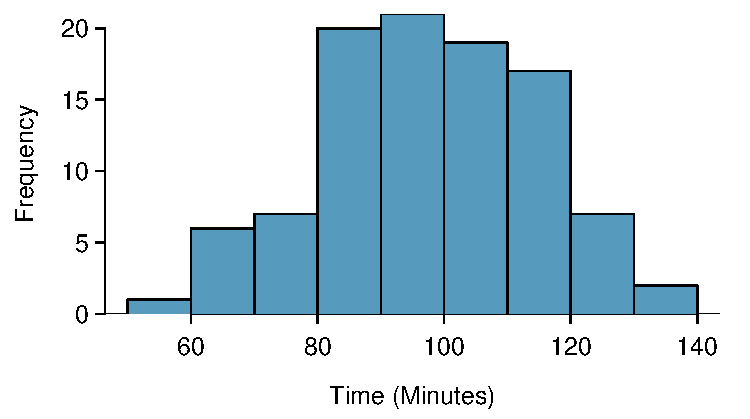
\includegraphics[width=0.65\textwidth]{ch_inference_for_means/figures/run10SampTimeHistogram/run17SampTimeHistogram} 
\caption{A histogram of \var{time} for the sample of 2017 Cherry Blossom Race participants.}
\label{run17SampTimeHistogram}
\end{figure}


\begin{examplewrap}
\begin{nexample}
{What are appropriate hypotheses for this context?}
We know that the average run time for all runners in 2006 was \cherryblossomnull{} minutes.  We have a sample of times from the 2017 race.  We are interested in whether the average run time has \emph{changed}, so we will use a two-sided $H_A$.\\
\\
Let $\mu$ represent the average 10-mile run time of all participants in 2017,\mbox{ which is unknown to us.}
\\
\\
$H_0$: $\mu = \cherryblossomnull{}$ minutes. \mbox{The average run time of all participants in 2017 was \cherryblossomnull{} min.}
\\$H_A$: $\mu \neq \cherryblossomnull{}$ minutes. \mbox{The average run time of all participants in 2017 was not \cherryblossomnull{} min.}
\end{nexample}
\end{examplewrap}

The data come from a random sample from a large population, so the observations are independent. Do we need to check for skew in the data? No -- with a sample size of \cherryblossomn{}, well over 30, the Central Limit Theorem tells us that the sampling distribution of $\bar{x}$ will be nearly normal.

With independence satisfied and slight skew not a concern for this large of a sample, we can proceed with performing a hypothesis test using the $t$-distribution.

The sample mean and sample standard deviation of the \cherryblossomn{} runners from the 2017 Cherry Blossom Race are \cherryblossommean{} and \cherryblossomsd{} minutes, respectively. We want to know whether the observed sample mean of \cherryblossommean{} is far enough away from \cherryblossomnull{} to provide convincing evidence of a real difference, or if it is within the realm of expected variation for a sample of size \cherryblossomn{}.  

\D{\newpage}

To answer this question we will find the test statistic and p-value for the hypothesis test.  Since we will be using a sample standard deviation in our calculation of the test statistic, we will need to use a $t$-distribution, just as we did with confidence intervals for a mean.  We call the test statistic a $T$-statistic.  It has the same general form as a Z-statistic.
\begin{align*}
T = \frac{\text{point estimate } - \text{null value}}{SE\text{ of estimate}}
\end{align*}

As we saw before, when carrying out inference on a single mean, the degrees of freedom is given by $n-1$.  


\begin{onebox}{The T-statistic}
The \term{T-statistic} (or T-score) is analogous to a Z-statistic (or Z-score).  Both represent how many standard errors the observed value is from the null value.
\end{onebox}


\begin{examplewrap}
\begin{nexample}{Calculate the test statistic, degrees of freedom, and p-value for this test.}
Here, our point estimate is the sample mean, $\bar{x}=\cherryblossommean{}$ minutes.  
\\
\\
The $SE$ of the sample mean is given by $\frac{s}{\sqrt{n}}$, so the \mbox{$SE$ of estimate = $\frac{\cherryblossomsd{}}{ \sqrt{\cherryblossomn{}}} = \cherryblossomse{}$ minutes.}

\begin{align*}
 T = \frac{\cherryblossommean{} - \cherryblossomnull{}}{\cherryblossomse{}} = \cherryblossomt{} \qquad df=\cherryblossomn{}-1=99
\end{align*}
Using a calculator, we find that the area above \cherryblossomt{} under the $t$-distribution with 99 degrees of freedom is 0.01.  Because this is a two-tailed test, we double this.  So the p-value = $2\times 0.01 = 0.02.$
\end{nexample}
\end{examplewrap}

\begin{examplewrap}
\begin{nexample}{Does the data provide sufficient evidence that the average Cherry Blossom Run time in 2017 is different than in 2006?}
This depends upon the desired significance level.  Since the p-value = 0.02 $< 0.05$, there is sufficient evidence at the 5\% significance level.  However, as the p-value of 0.02 $> 0.01$, there is not sufficient evidence at the 1\% significance level.
\end{nexample}
\end{examplewrap}


\begin{examplewrap}
\begin{nexample}{Would you expect the hypothesized value of \cherryblossomnull{} to fall inside or outside of a 95\% confidence interval?  What about a 99\% confidence interval?} 
Because the hypothesized value of \cherryblossomnull{} was rejected by the two-sided $\alpha=0.05$ test, we would expect it to be outside the 95\% confidence interval.  However, because the hypothesized value of \cherryblossomnull{} was not rejected by the two-sided $\alpha=0.01$ test, we would expect it to fall inside the (wider) 99\% confidence interval.  
\end{nexample}
\end{examplewrap}


\begin{onebox}{Hypothesis test for a mean}
To carry out a complete hypothesis test to test the claim that a single mean $\mu$ is equal to a null value $\mu_0$,
\\
\\
\inferencestep{Identify} Identify the hypotheses and the significance level, $\alpha$.\vspace{-1mm}
\begin{itemize}
\setlength{\itemsep}{0mm}
\item[] $H_0$: $\mu = \mu_0$  
\item[]  $H_A$: $\mu \ne \mu_0$;  \quad $H_A$: $\mu > \mu_0$; \quad or \quad $H_A$: $\mu < \mu_0$ 
\end{itemize} 
\inferencestep{Choose} Choose the appropriate test procedure and identify it by name. \vspace{-1mm}
\begin{itemize}
\item[] Here we choose the \term{1-sample $t$-test}.
\end{itemize}
 \inferencestep{Check} Check conditions for the sampling distribution of $\bar{x}$ to be nearly normal.\vspace{-1mm}
\begin{itemize}
\setlength{\itemsep}{0mm}
\item[] 1. Data come from a random sample or random process.
\item[] 2. The sample size $n\ge 30$ or the population distribution is nearly normal.
\item[] \quad \ If the sample size is less than 30 and the population distribution is unknown, check 
\item[] \quad \ for strong skew or outliers in the data.  If neither is found, then the condition that the 
\item[] \quad \ population is nearly normal is considered reasonable.  
\end{itemize}
 \inferencestep{Calculate} Calculate the $t$-statistic, $df$, and p-value.
\begin{itemize}
\item[] $T = \frac{\text{point estimate } - \text{ null value}}{SE \text{ of estimate}}$,  \quad $df=n-1$
\begin{itemize}
\item[] point estimate:  the sample mean $\bar{x}$
\item[] $SE$ of estimate:  $\frac{s}{\sqrt{n}}$
\item[] null value: $\mu_0$
\end{itemize}
\item[] p-value = (based on the $t$-statistic, the $df$, and the direction of $H_A$)
\end{itemize}
 \inferencestep{Conclude} Compare the p-value to $\alpha$, and draw a conclusion in context.\vspace{-1mm}
\begin{itemize}
\item[] If the p-value is $< \alpha$, reject $H_0$; there is sufficient evidence that [$H_A$ in context]. 
\item[] If the p-value is $> \alpha$, do not reject $H_0$; there is not sufficient evidence that [$H_A$ in context].
\end{itemize}\end{onebox}


\begin{examplewrap}
\begin{nexample}
{Recall the example involving the mercury content in croaker white fish (Pacific). Based on a sample of size 15, a sample mean and standard deviation were computed as 0.287 and 0.069 ppm (parts per million), respectively. Carry out an appropriate test to determine if 0.25 is a reasonable value for the average mercury content of croaker white fish (Pacific).  Use the five step method to organize your work.}

\begin{description}
\item[\inferencestep{Identify}]  We will test the following hypotheses at the $\alpha=0.05$ significance level.\\
$H_0$: $\mu=0.25$   \\
$H_A$: $\mu \ne 0.25$ \quad The mean mercury content is not 0.25 ppm.\\
 
\item[\inferencestep{Choose}] Because we are hypothesizing about a single mean we choose the \mbox{1-sample $t$-test.}
\item[\inferencestep{Check}]  The conditions were checked previously, namely -- the data come from a random sample, and because $n$ is less than 30, we verified that there is no strong skew or outliers in the data, so the assumption that the population distribution of mercury is nearly normally distributed is reasonable.  
\item[ \inferencestep{Calculate} ]  We will calculate the $t$-statistic and the p-value.
\begin{align*}
T = \frac{\text{point estimate } - \text{ null value}}{SE \text{ of estimate}}
\end{align*}

The point estimate is the sample mean:  $\bar{x}$ =  0.287 \\
\\
The $SE$ of the sample mean is:  $\frac{s}{\sqrt{n}} = \frac{0.069}{\sqrt{15}} = 0.0178$\\ 
\\
The null value is the value hypothesized for the parameter in $H_0$, which is 0.25.\\
\\
For the 1-sample $t$-test, $df = n-1$.
\\
\begin{align*}
T = \frac{0.287 - 0.25}{0.0178} = 2.07 \qquad df= 15-1=14
\end{align*}
Because $H_A$ is a two-tailed test ( $\ne$ ), the p-value corresponds to the area to the right of $t=2.07$ plus the area to the left of $t=-2.07$ under the $t$-distribution with 14 degrees of freedom.  The p-value = $2\times 0.029 = 0.058$.  

\item[\inferencestep{Conclude}]  The p-value of $0.058 > 0.05$, so we do not reject the null hypothesis. We do not have sufficient evidence that the average mercury content in croaker white fish (Pacific) is not 0.25.
\end{description}

\end{nexample}
\end{examplewrap}

\begin{exercisewrap}
\begin{nexercise}Recall that the 95\% confidence interval for the average mercury content in croaker white fish was (0.249, 0.325). Discuss whether the conclusion of the hypothesis test in the previous example is consistent or inconsistent with the conclusion of the confidence interval.\footnotemark
\end{nexercise}
\end{exercisewrap}
\footnotetext{It is consistent because 0.25 is located (just barely) inside the confidence interval, so it is considered a reasonable value. Our hypothesis test did not reject the hypothesis that $\mu=0.25$, also implying that it is a reasonable value. Note that the p-value was just over the cutoff of 0.05. This is consistent with the value of 0.25 being just inside the confidence interval.  Also note that the hypothesis test did not \emph{prove} that $\mu=0.25$.  The value 0.25 is just one of many reasonable values for the true mean.}


\D{\newpage}

%%
\subsection[Calculator: 1-sample $t$-test]{Calculator: 1-sample \pmb{$t$}-test}
\label{1SampTtest}

\begin{onebox}{\videohref{ti84_1_mean_HT} TI-83/84: 1-sample T-test}
Use \calctext{STAT}, \calctext{TESTS}, \calctext{T-Test}.
\begin{enumerate}
\setlength{\itemsep}{0mm}
\item Choose \calcbutton{STAT}.
\item Right arrow to \calctext{TESTS}.
\item Down arrow and choose \calctext{2:T-Test}.
\item Choose \calctext{Data} if you have all the data or \calctext{Stats} if you have the mean and standard deviation.
\item Let $\calctextmath{\mu_0}$ be the null or hypothesized value of $\mu$.
\begin{itemize}
\item If you choose \calctext{Data}, let \calctext{List} be \calctext{L1} or the list in which you entered your data (don't forget to enter the data!) and let \calctext{Freq} be \calctext{1}.
\item If you choose \calctext{Stats}, enter the mean, $SD$, and sample size.
\end{itemize}
\item Choose $\calctextmath{\ne}$, $\calctextmath{<}$, or $\calctextmath{>}$ to correspond to $H_A$.
\item Choose \calctext{Calculate} and hit \calcbutton{ENTER}, which returns: \\
\begin{tabular}{ll l ll}
\calctext{t} & t statistic &\quad&
	\calctext{Sx} & the sample standard deviation \\
\calctext{p} & p-value &&
	\calctext{n} & the sample size \\
$\calctextmath{\bar{x}}$ & the sample mean

\end{tabular}
\end{enumerate}
\end{onebox}

\begin{onebox}{\videohref{casio_1_mean_inference} Casio fx-9750GII: 1-sample T-test}
\begin{enumerate}
\setlength{\itemsep}{0mm}
\item Navigate to \calctext{STAT} (\calcbutton{MENU} button, then hit the \calcbutton{2} button or select \calctext{STAT}).
\item If necessary, enter the data into a list.
\item Choose the \calctext{TEST} option (\calcbutton{F3} button).
\item Choose the \calctext{t} option (\calcbutton{F2} button).
\item Choose the \calctext{1-S} option (\calcbutton{F1} button).
\item Choose either the \calctext{Var} option (\calcbutton{F2}) or enter the data in using the \calctext{List} option.
\item Specify the test details:
  \begin{itemize}
  \setlength{\itemsep}{0mm}
  \item Specify the sidedness of the test using the \calcbutton{F1}, \calcbutton{F2}, and \calcbutton{F3} keys.
  \item Enter the null value, $\calctextmath{\mu}$\calctext{0}.
  \item If using the \calctext{Var} option, enter the summary statistics. If using \calctext{List}, specify the list and leave \calctext{Freq} values at \calctext{1}.
  \end{itemize}
\item Hit the \calcbutton{EXE} button, which returns \\[1mm]
\begin{tabular}{ll l ll}
& alternative hypothesis &\hspace{5mm}&
	$\calctextmath{\bar{x}}$ & sample mean \\
\calctext{t} & T statistic &&
	\calctext{sx} & sample standard deviation \\
\calctext{p} & p-value &&
	\calctext{n} & sample size
\end{tabular}
\end{enumerate}
\end{onebox}

\begin{exercisewrap}
\begin{nexercise}
The average time for all runners who finished the Cherry Blossom Run in 2006 was \cherryblossomnull{} minutes. In 2017, the average time for \cherryblossomn{} randomly selected participants was \cherryblossommean{}, with a standard deviation of \cherryblossomsd{} minutes. Use a calculator to find the $T$-statistic and p-value for the appropriate test to see if the average time for the participants in 2017 is different than it was in 2006.\footnotemark
\end{nexercise}
\end{exercisewrap}
\footnotetext{Choose \calctext{T-Test} or equivalent.  Let $\calctextmath{\mu_0}$ be \cherryblossomnull{}. $\calctextmath{\bar{x}}$ is \cherryblossommean{}, $\calctextmath{S_x}$ is \cherryblossomsd{}, and $\calctext{n} = \cherryblossomn{}$.  Choose $\calctextmath{\neq}$ to correspond to $H_A$. We get $\calctextmath{t} =2.353$ and the p-value \calctext{p} = 0.021.}



\D{\newpage}

%%
\subsection*{Section summary}
\begin{itemize} 
\item The $t$-distribution.\vspace{-1mm}
\begin{itemize}
\setlength{\itemsep}{0mm}
\item When calculating a test statistic for a mean, using the sample standard deviation in place of the population standard deviation gives rise to a new distribution called the $t$-distribution.  

\item As the sample size and degrees of freedom increase, $s$ becomes a more stable estimate of $\sigma$, and the corresponding $t$-distribution has smaller spread.  

\item As the degrees of freedom go to $\infty$, the $t$-distribution approaches the normal distribution.  This is why we can use the $t$-table at $df=\infty$ to find the value of $z^{\star}$.
\end{itemize}

\item When carrying out inference for a single mean, we use the $t$-distribution with $n-1$ degrees of freedom.

\item When there is one sample and the parameter of interest is a single mean:
\begin{itemize}
\item Estimate $\mu$ at the C\% confidence level using a \term{1-sample t-interval}.
\item Test $H_0$: $\mu=\mu_0$ at the $\alpha$ significance level using a \term{1-sample t-test}. 
\end{itemize}

\item The conditions for the one sample $t$-interval and $t$-test are the same.  
\begin{itemize}
\item[1.] The data come from a random sample or random process.
\item[2.]  The sample size $n\ge 30$ or the population distribution is nearly normal.
\item[]  If the sample size is less than 30 and the population distribution is unknown, check for strong skew or outliers in the data.  If neither is found, then the condition that the population distribution is nearly normal is considered reasonable.
\end{itemize}

\item When the conditions are met, we calculate the confidence interval and the test statistic as we did in the previous chapter, except that we use $t^{\star}$ for the critical value and we use $T$ for the test statistic.

\begin{itemize}
\setlength{\itemsep}{2mm}
\item[] Confidence interval:\ \  $\text{point estimate}\ \pm\ t^{\star} \times SE\ \text{of estimate}$
\item[] Test statistic:  $T = \frac{\text{point estimate } - \text{ null value}}{SE \text{ of estimate}}$ 
\end{itemize}
Here the point estimate is the sample mean: $\bar{x}$.
\item[] The $SE$ of estimate is the $SE$ of the sample mean: $\frac{s}{\sqrt{n}}$.
\item[] The degrees of freedom is given by $df = n-1$.

\item To calculate the minimum sample size required to estimate a mean with C\% confidence and a margin of error no greater than $m$, we set up an inequality as follows: 
\begin{align*}
z^{\star}\frac{\sigma}{\sqrt{n}}\leq m
\end{align*}
$z^{\star}$ depends on the desired confidence level and $\sigma$ is the standard deviation associated with the population. We solve for the sample size, $n$.  Always round the answer up to the next \emph{integer}, since $n$ refers to a number of people or things. 

\end{itemize}


%%%%%Section exercises
{\exercisesheader{}

% 1

\eoce{\qt{Identify the critical $t$\label{identify_critical_t}} \videohref{ahss_eoce_sol-identify_critical_t}\ \ An independent random 
sample is selected from an approximately normal population with unknown 
standard deviation. Find the degrees of freedom and the critical $t$-value 
(t$^\star$) for the given sample size and confidence level.
%\begin{multicols}{4}
\begin{parts}
\item $n = 6$, CL = 90\%
\item $n = 21$, CL = 98\%
\item $n = 29$, CL = 95\%
\item $n = 12$, CL = 99\%
\end{parts}
%\end{multicols}
}{}

% 2

\eoce{\qt{$t$-distribution\label{t_distribution}}
The figure on the right shows three 
unimodal and symmetric curves:
the standard normal (z) distribution,
the $t$-distribution with 5 degrees of freedom,
and the $t$-distribution with 1 degree of freedom.
Determine which is which, and explain your reasoning.
\begin{center}
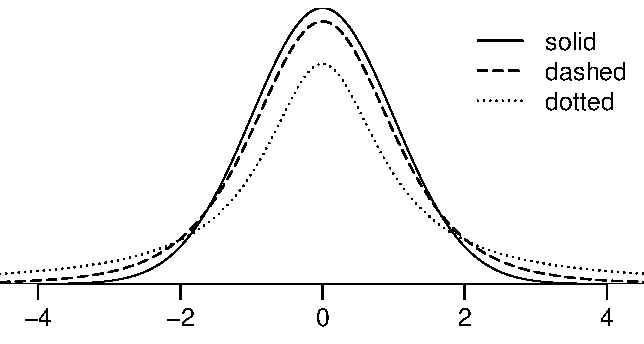
\includegraphics[width=0.4\textwidth]{ch_inference_for_means/figures/eoce/t_distribution/t_distribution}
\end{center}
}{}

% 3

\eoce{\qt{Find the p-value, Part I\label{find_T_pval_1_2_sided}}
An independent random sample 
is selected from an approximately normal population
with an unknown standard 
deviation.
Find the p-value for the given sample size and test statistic.
Also determine if the null hypothesis would be rejected at 
$\alpha = 0.05$.
\begin{parts}
\item $n = 11$, $T = 1.91$
\item $n = 17$, $T = -3.45$
\item $n = 7$, $T = 0.83$
\item $n = 28$, $T = 2.13$
\end{parts}
}{}

% 4

\eoce{\qt{Find the p-value, Part II\label{find_T_pval_2_2_sided}}
An independent random sample 
is selected from an approximately normal population
with an unknown standard 
deviation.
Find the p-value for the given sample size and test statistic.
Also determine if the null hypothesis would be rejected at 
$\alpha = 0.01$.
\begin{parts}
\item $n = 26$, $T = 2.485$
\item $n = 18$, $T = 0.5$
\end{parts}
}{}

% 5

\eoce{\qt{Working backwards, Part I\label{work_backwards_1}} A 95\% confidence 
interval for a population mean, $\mu$, is given as (18.985, 21.015). This 
confidence interval is based on a simple random sample of 36 observations. 
Calculate the sample mean and standard deviation. Assume that all conditions 
necessary for inference are satisfied. Use the $t$-distribution in any 
calculations.
}{}

% 6

\eoce{\qt{Working backwards, Part II\label{work_backwards_2}} A 90\% confidence 
interval for a population mean is (65, 77). The population distribution is 
approximately normal and the population standard deviation is unknown. This 
confidence interval is based on a simple random sample of 25 observations. 
Calculate the sample mean, the margin of error, and the sample standard 
deviation.
}{}

% 7

\eoce{\qt{Sleep habits of New Yorkers\label{ny_sleep_habits_2_sided}}
New York is known as 
``the city that never sleeps".
A random sample of 25 New Yorkers were asked how 
much sleep they get per night.
Statistical summaries of these data are shown 
below.
The point estimate suggests New Yorkers sleep less than
8~hours a night on average.
Is the result statistically significant?
\begin{center}
\begin{tabular}{rrrrrr}
 \hline
n   & $\bar{x}$ & s     & min   & max \\ 
 \hline
25  & 7.73      & 0.77  & 6.17  & 9.78 \\ 
  \hline
\end{tabular}
\end{center}

\begin{parts}
\item Write the hypotheses in symbols and in words.
\item Check conditions, then calculate the test statistic, $T$, and the 
associated degrees of freedom.
\item Find and interpret the p-value in this context. Drawing a picture may be 
helpful.
\item What is the conclusion of the hypothesis test?
\item If you were to construct a 90\% confidence interval that corresponded to 
this hypothesis test, would you expect 8 hours to be in the interval?
\end{parts}
}{}

% 8

\eoce{\qt{Heights of adults\label{adult_heights}}
Researchers studying anthropometry 
collected body girth measurements and skeletal diameter measurements, as well as 
age, weight, height and gender, for 507 physically active individuals. The 
histogram below shows the sample distribution of heights in centimeters. 
\footfullcite{Heinz:2003} \\
\begin{minipage}[c]{0.75\textwidth}
\begin{center}
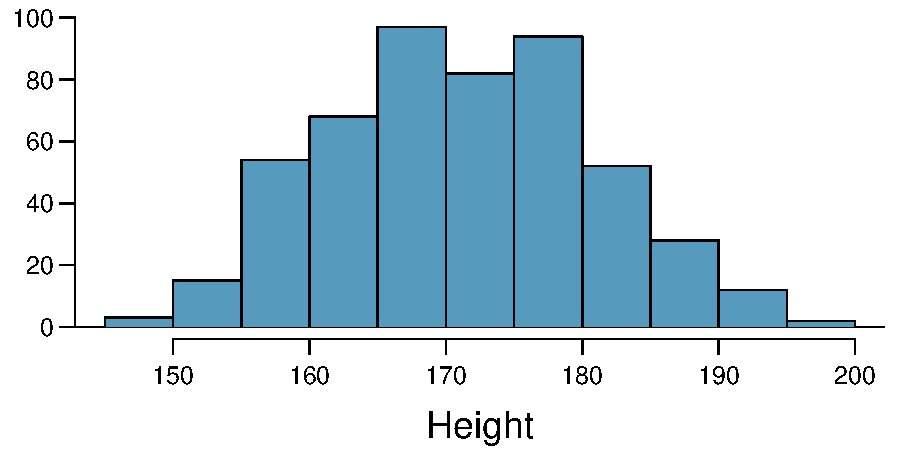
\includegraphics[width=\textwidth]{ch_inference_for_means/figures/eoce/adult_heights/adult_heights_hist.pdf}
\end{center}
\end{minipage}
\begin{minipage}[c]{0.23\textwidth}
\begin{center}
\begin{tabular}{l|r l}
Min     & 147.2 \\
Q1      & 163.8 \\
Median  & 170.3 \\
Mean    & 171.1 \\
SD      &  9.4 \\
Q3      & 177.8 \\
Max     & 198.1 \\
\end{tabular}
\end{center}
\end{minipage}
\begin{parts}
\item What is the point estimate for the average height of active individuals? 
What about the median?
\item What is the point estimate for the standard deviation of the heights of 
active individuals? What about the IQR?
\item Is a person who is 1m 80cm (180 cm) tall considered unusually tall? And is 
a person who is 1m 55cm (155cm) considered unusually short? Explain your 
reasoning.
\item The researchers take another random sample of physically active 
individuals. Would you expect the mean and the standard deviation of this new 
sample to be the ones given above? Explain your reasoning.
\item The sample means obtained are point estimates for the mean height of all 
active individuals, if the sample of individuals is equivalent to a simple 
random sample.
What measure do we use to quantify the variability of such an estimate?
Compute 
this quantity using the data from the original sample under the condition that 
the data are a simple random sample. 
\end{parts}
}{}

% 9

\eoce{\qt{Find the mean\label{find_mean_2_sided}}
You are given the following hypotheses:
\begin{align*}
H_0&: \mu = 60 \\
H_A&: \mu \neq 60
\end{align*}
We know that the sample standard deviation is 8
and the sample size is 20.
For what sample mean would the p-value be equal to 0.05?
Assume that all conditions necessary for inference are satisfied.
}{}

% 10

\eoce{\qt{$t^\star$ vs. $z^\star$\label{critical_t_vs_z}} For a given confidence 
level, $t^{\star}_{df}$ is larger than $z^{\star}$. Explain how $t^{*}_{df}$ 
being slightly larger than $z^{*}$ affects the width of the confidence interval.
}{}

% 11

\eoce{\qt{Play the piano\label{play_piano_one_sided}} \videohref{ahss_eoce_sol-play_piano}\ \ 
Georgianna claims that in a small city 
renowned for its music school, the average child takes at least 5 years of 
piano lessons. We have a random sample of 30 children from the city, with a 
mean of 4.6 years of piano lessons and a standard deviation of 2.2 years.
\begin{parts}
\item Use a hypothesis test to determine if there is sufficient evidence against Georgianna's claim.
\item Construct a 95\% confidence interval for the number of years students in this city take piano lessons, and interpret it in context of the data.
\item Do your results from the hypothesis test and the confidence interval agree? Explain your reasoning.
\end{parts}
}{}

% 12

\eoce{\qt{Auto exhaust and
    lead exposure\label{auto_exhaust_lead_exposure_2_sided}} 
Researchers interested in lead exposure due to car exhaust
sampled the blood of 52 police officers subjected to constant
inhalation of automobile exhaust fumes while working traffic
enforcement in a primarily urban environment.
The blood samples of these officers had an average lead
concentration of 124.32 $\mu$g/l and a SD of 37.74 $\mu$g/l;
a previous study of individuals from a nearby suburb,
with no history of exposure, found an average blood level
concentration 
of 35 $\mu$g/l.\footfullcite{Mortada:2000}
\begin{parts}
\item
    Write down the hypotheses that would be appropriate for
    testing if the police officers appear to have been exposed
    to a different concentration of lead.
\item\label{auto_exhaust_lead_exposure_2_sided_cond}
    Explicitly state and check all conditions necessary for
    inference on these data.
\item
    Regardless of your answers in
    part~(\ref{auto_exhaust_lead_exposure_2_sided_cond}),
    test the hypothesis that the downtown police officers have
    a higher lead exposure than the group in the previous study.
    Interpret your results in context.
\end{parts}
}{}

% 13

\eoce{\qt{Car insurance savings\label{car_insurance_savings}} \videohref{ahss_eoce_sol-car_insurance_savings}\ \ 
A market researcher wants to evaluate car insurance savings
at a competing company.
Based on past studies he is assuming that the standard
deviation of savings is \$100.
He wants to collect data such that he can get a margin of
error of no more than \$10 at a 95\% confidence level.
How large of a sample should he collect?
}{}

% 14

\eoce{\qt{SAT scores\label{sat_scores_CI}}
The standard deviation of SAT scores for students at
a particular Ivy League college is 250 points.
Two statistics students, Raina and Luke, want to estimate
the average SAT score of students at this college as part
of a class project.
They want their margin of error to be no more than 25 points.
\begin{parts}
\item
    Raina wants to use a 90\% confidence interval.
    How large a sample should she collect?
\item
    Luke wants to use a 99\% confidence interval.
    Without calculating the actual sample size, determine
    whether his sample should be larger or smaller
    than Raina's, and explain your reasoning.
\item
    Calculate the minimum required sample size for Luke.
\end{parts}
}{}
}


%_______________________________________
\section[Inference for paired data]{Inference for paired data }

\label{pairedData}

\index{paired data|(}
\index{data!textbooks|(}

\sectionintro{
\noindent%
When we have two observations on each person or each case, we can answer questions such as the following:
\begin{itemize}
\item Do students do better on reading or writing sections of standardized tests?
\item How do the number of days with temperature above 90\textdegree{}F compare between 1948 and 2018?
\item Are Amazon textbook prices lower than the college bookstore prices?  If so, how much lower, on average?
\end{itemize}


%%
\subsection*{Learning objectives}

\begin{enumerate}
\setlength{\itemsep}{0mm}
\item Distinguish between paired and unpaired data.  

\item Recognize that inference procedures for paired data use the same one-sample $t$-procedures as in the previous section, and that these procedures are applied to the \emph{differences} of the paired observations.

\item Carry out a complete hypothesis test for paired differences.

\item Carry out a complete confidence interval procedure for paired differences.

\end{enumerate}
}

%%
\subsection{Paired observations and samples}



\newcommand{\uclabookN}{68}
\newcommand{\uclabookM}{3.58}
\newcommand{\uclabookSD}{13.42}
\newcommand{\uclabookSE}{1.63}

\index{paired data|(}
\index{data!textbooks|(}

\noindent%
In the previous edition of this textbook,
we found that Amazon prices were, on average,
lower than those of the UCLA Bookstore for UCLA courses
in 2010.
It's been several years, and many stores have adapted
to the online market, so we wondered,
how is the UCLA Bookstore doing today?

We sampled 201 UCLA courses.
Of those, \uclabookN{}
required books that could be found on Amazon.
A~portion of the data set from these courses
is shown in Figure~\ref{textbooksDF},
where prices are in U.S. dollars.

\begin{figure}[h]
\centering
\begin{tabular}{r ll ccc}
  \hline
 & subject &
     course\us{}number &
     bookstore &
     amazon &
     price\us{}difference \\ 
  \hline
  1 & American Indian Studies & M10 & 47.97 & 47.45 & 0.52 \\ 
  2 & Anthropology & 2 & 14.26 & 13.55 & 0.71 \\ 
  3 & Arts and Architecture & 10 & 13.50 & 12.53 & 0.97 \\
  $\vdots$ & $\vdots$ & $\vdots$ & $\vdots$ & $\vdots$ & $\vdots$ \\
  67 & Korean & 1 & 24.96 & 23.79 & 1.17 \\ 
  68 & Jewish Studies & M10 & 35.96 & 32.40 & 3.56 \\
  \hline
\end{tabular}
\caption{Five cases of the \data{textbooks} data set.}
\label{textbooksDF}
\end{figure}
% library(openintro); library(xtable); library(dplyr); d <- select(ucla_textbooks_f18, subject, course_num, bookstore_new, amazon_new); d$price_diff <- d$bookstore_new - d$amazon_new; d <- subset(d, !is.na(bookstore_new) & !is.na(amazon_new)); rownames(d) <- NULL; xtable(d[c(1:3, nrow(d) - 1:0),])

Each textbook has two corresponding prices in the data set:
one for the UCLA Bookstore and one for Amazon.
Therefore, each textbook price from the UCLA bookstore
has a natural correspondence with a textbook price from
Amazon.
When two sets of observations have this special
correspondence, they are said to be \term{paired}.

\begin{onebox}{Paired data}
  Two sets of observations are \emph{paired} if each
  observation in one set has a special correspondence
  or connection with exactly one observation in the other
  data set.
\end{onebox}

To analyze paired data, it is often useful to look
at the difference in outcomes of each pair of observations.
In the \data{textbook} data set, we look at the differences
in prices, which is represented as the \data{diff} variable.
Here, for each book, the differences are taken as
\begin{eqnarray*}
\text{UCLA Bookstore price} - \text{Amazon price}
\end{eqnarray*}

It is important that we always subtract using
a consistent order;
here Amazon prices are always subtracted from UCLA prices.
A histogram of these differences is shown in
Figure~\ref{diffInTextbookPricesF18}.
Using differences between paired observations
is a common and useful way to analyze paired data.

\begin{figure}
\centering
\oiRedirect{tableau-hist-textbookdiff-summ}{
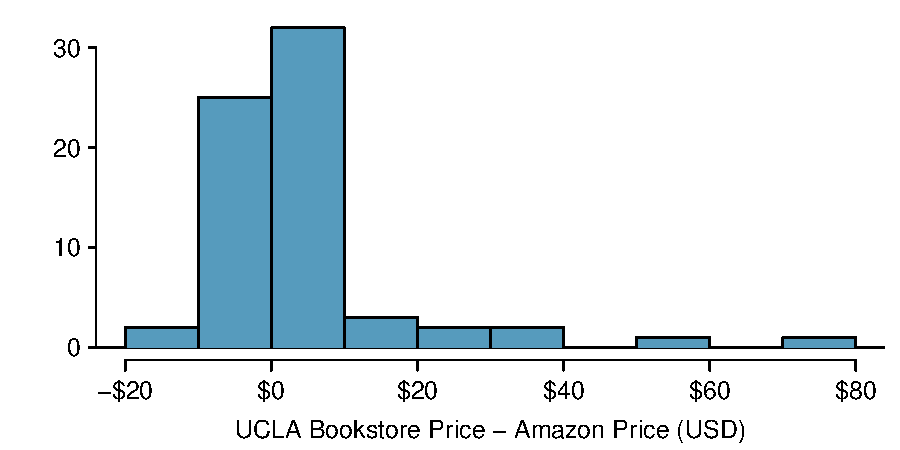
\includegraphics[width=0.73\textwidth]{ch_inference_for_means/figures/textbooksF18/diffInTextbookPricesF18}}
\caption{Histogram of the difference in price for
    each book sampled.
    These data are very strongly skewed.
    \index{skew!example: very strong}. Explore this data set on Tableau Public\tableauhref{tableau-hist-textbookdiff-summ}.}
\label{diffInTextbookPricesF18}
\end{figure}

\begin{exercisewrap}
\begin{nexercise}
The first difference shown in Figure~\ref{textbooksDF}
is computed as: $47.97 - 47.45 = 0.52$.
What does this difference tell us about the price for this textbook on Amazon versus the UCLA bookstore?\footnotemark
\end{nexercise}
\end{exercisewrap}
\footnotetext{The difference is taken as UCLA Bookstore price $-$ Amazon price.  Because the difference is positive, it tells us that the UCLA Bookstore price was \emph{greater} for this textbook.  In fact, it was $\$0.52$, or 52 cents, more expensive at the UCLA bookstore than on Amazon.  }


%%
\subsection{Hypothesis tests for paired data}

To analyze a paired data set,
we simply analyze the differences.
We can use the same $t$-distribution techniques
we applied in the last section.

\begin{figure}[hh]
\centering
\begin{tabular}{ccccc}
\hline
$n_{_{\text{\emph{diff}}}}$	&\hspace{3mm}& $\bar{x}_{_{\text{\emph{diff}}}}$	&\hspace{3mm}& $s_{_{\text{\emph{diff}}}}$ \vspace{1mm}\\
\uclabookN{}  && \uclabookM{}  && \uclabookSD{} \\
\hline
\end{tabular}
\caption{Summary statistics for the price differences.
    There were 68 books, so there are \uclabookN{}
    differences.}
\label{textbooksSummaryStats}
\end{figure}

\D{\newpage}

We will set up and implement a hypothesis test to determine whether, on average, there is a difference in textbook prices between Amazon and the UCLA bookstore.
\label{htForDiffInUCLAAndAmazonTextbookPrices}
We are considering two scenarios: there is no difference in prices or there is some difference in prices.
\begin{itemize}
\setlength{\itemsep}{0mm}
\item[$H_0$:] $\mu_{\text{\emph{diff}}}=0$. On average, there is no difference in textbook prices.
\item[$H_A$:] $\mu_{\text{\emph{diff}}} \neq 0$. On average, there is some difference in textbook prices.
\end{itemize}

Can the $t$-distribution be used for this application?
The observations are based on a random sample from a large population,
so independence is reasonable.
While the distribution of the data is very strongly skewed,
we do have $n = \uclabookN{}$ observations.  This sample size is large enough that we do not have to worry about whether the population distribution for difference in price might be nearly normal or not.
Because the conditions are satisfied,
we can use the $t$-distribution to this setting.

We compute the standard error associated with
$\bar{x}_{\text{\emph{diff}}}$ using the standard
deviation of the differences
($s_{_{\text{\emph{diff}}}} = \uclabookSD{}$)
and the number of differences
($n_{_{\text{\emph{diff}}}} = \uclabookN{}$):
\begin{align*}
SE_{\bar{x}_{\text{\emph{diff}}}}
  = \frac{s_{\text{\emph{diff}}}}{\sqrt{n_{\text{\emph{diff}}}}}
  = \frac{\uclabookSD{}}{\sqrt{\uclabookN{}}} = \uclabookSE{}
\end{align*}

Next we compute the test statistic.  The point estimate is the observed value of $\bar{x}_{\text{\emph{diff}}}$.  The null value is the value hypothesized under the null hypothesis.  Here, the null hypothesis is that the true mean of the differences is 0.  
\begin{align*}
T
  = \frac{\text{point estimate} - \text{null value}}
      {SE \text{ of estimate}}
  = \frac{\uclabookM{} - 0}{\uclabookSE{}} = 2.20
\end{align*}
The degrees of freedom are $df = \uclabookN{} - 1 = 67$.
To visualize the p-value, the sampling distribution
of $\bar{x}_{\text{\emph{diff}}}$ is drawn as though
$H_0$ is true.  This is shown in
Figure~\ref{textbooksF18HTTails}.  Because this is a two-sided test, the p-value corresponds to the area in both tails.  Using statistical software, we find the area in the tails to be 0.0312.

Because the p-value of 0.0312 is less than 0.05,
we reject the null hypothesis.  We have evidence that, on average, there is a difference in textbook prices.  In particular, we can say that, on average, Amazon prices are lower than the
UCLA Bookstore prices for UCLA course textbooks.


\begin{figure}[h]
\centering
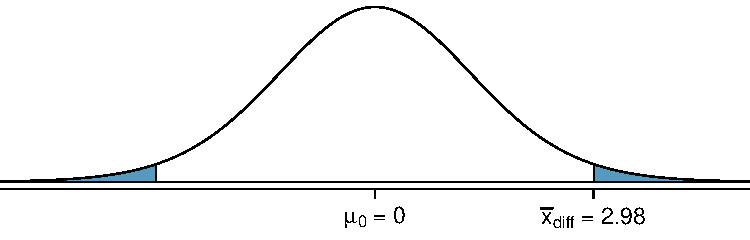
\includegraphics[width=0.65\textwidth]{ch_inference_for_means/figures/textbooksF18/textbooksF18HTTails}
\caption{Sampling distribution for the mean difference in book prices, if the true average difference is zero.}
\label{textbooksF18HTTails}
\end{figure}

\begin{examplewrap}
\begin{nexample}{We have evidence to conclude Amazon is,
on average, less expensive. Does this mean that UCLA students should always buy their books
on Amazon?}No. The fact that Amazon is, on average, less expensive, does not imply that it is less expensive for \emph{every} textbook.  Examining the distribution shown in
  Figure~\ref{diffInTextbookPricesF18}, we see that there are certainly a handful of cases where
  Amazon prices are much lower than the UCLA Bookstore's,
  which suggests it is worth checking Amazon
  or other online sites before purchasing.
  However, in many cases the Amazon price is
  \emph{above} what the UCLA Bookstore charges,
  and most of the time the price isn't that different.  
\end{nexample}
\end{examplewrap}
  For reference, this is a very different result
  from what we (the authors) had seen in a similar
  data set from 2010.
  At that time, Amazon prices were almost uniformly
  lower than those of the UCLA Bookstore's and by
  a large margin, making the case to use Amazon over
  the UCLA Bookstore quite compelling at that time.

\index{data!textbooks|)}
\index{paired data|)}







\begin{onebox}{Hypothesis test for paired data}
To carry out a complete hypothesis test to test the claim that a mean of differences $\mu_{\text{\emph{diff}}}$ is equal to 0,
\\
\\
\inferencestep{Identify} Identify the hypotheses and the significance level, $\alpha$.\vspace{-1mm}
\begin{itemize}
\setlength{\itemsep}{0mm}
\item[] $H_0$: $\mu_{\text{\emph{diff}}} = 0$  
\item[]  $H_A$: $\mu_{\text{\emph{diff}}} \ne 0$;  \quad $H_A$: $\mu_{\text{\emph{diff}}} > 0$; \quad or \quad $H_A$: $\mu_{\text{\emph{diff}}} < 0$ 
\end{itemize} 
\inferencestep{Choose} Choose the appropriate test procedure and identify it by name.  \vspace{-1mm}
\begin{itemize}
\item[] Here we choose the \term{matched pairs  $t$-test}.
\end{itemize}
 \inferencestep{Check} Check conditions for the sampling distribution of $\bar{x}_{\text{\emph{diff}}}$ to be nearly normal.\vspace{-1mm}
\begin{itemize}
\setlength{\itemsep}{0mm}
\item[] 1. There is paired data from a random sample or from a matched pairs experiment.
\item[] 2. $n_{\text{\emph{diff}}}\ge 30$ or the population of differences is nearly normal.
 \item[] \quad \  If the number of differences is less than 30 and the distribution of the population 
 \item[] \quad \ of differences is unknown, check for strong skew or outliers in the sample differences.
\item[] \quad \ If neither is found, then the condition that the population of differences is nearly normal 
\item[] \quad \ is considered reasonable.  
\end{itemize}
 \inferencestep{Calculate}  Calculate the $t$-statistic, $df$, and p-value.
\begin{itemize}
\item[] $T = \frac{\text{point estimate } - \text{ null value}}{SE \text{ of estimate}}$,  \quad $df=n_{\text{\emph{diff}}} -1$
\begin{itemize}
\item[] point estimate: the sample mean of differences $\bar{x}_{\text{\emph{diff}}} $
\item[] $SE$ of estimate:  $\frac{s_{\text{\emph{diff}}} }{\sqrt{n_{\text{\emph{diff}}} }}$
\item[] null value: $0$
\end{itemize}
\item[] p-value = (based on the $t$-statistic, the $df$, and the direction of $H_A$)
\end{itemize}
 \inferencestep{Conclude} Compare the p-value to $\alpha$, and draw a conclusion in context.\vspace{-1mm}
\begin{itemize}
\item[] If the p-value is $< \alpha$, reject $H_0$; there is sufficient evidence that [$H_A$ in context]. 
\item[] If the p-value is $> \alpha$, do not reject $H_0$; there is not sufficient evidence that [$H_A$ in context].
\end{itemize}\end{onebox}



\begin{figure}[h]
\centering
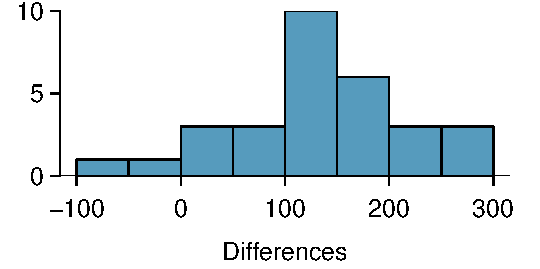
\includegraphics[width=0.5\textwidth]{ch_inference_for_means/figures/satImprovementHTDataHistogram/satImprovementHTDataHistogram}
\caption{SAT score after course - SAT score before course. }
\label{satImprovementHTDataHistogramrepeat}
\end{figure}

\begin{examplewrap}
\begin{nexample}
{An SAT preparation company claims that its students' scores improve by over 100 points on average after their course. A consumer group would like to evaluate this claim, and they collect data on a random sample of 30 students who took the class. Each of these students took the SAT before and after taking the company's course, so we have a difference in scores for each student. We will examine these differences $x_1=57$, $x_2=133$, ..., $x_{30}=140$ as a sample to evaluate the company's claim. The distribution of the differences, shown in Figure~\ref{satImprovementHTDataHistogramrepeat}, has a mean of 135.9 and a standard deviation of 82.2. Do these data provide convincing evidence to back up the company's claim?  Use the five step framework to organize your work.  
}
\begin{description}
\item[\inferencestep{Identify}] We will test the following hypotheses at the $\alpha=0.05$ level:\\
$H_0$: $\mu_{\text{\emph{diff}}} = 100$. Student scores improve by 100 points, on average.   \\
$H_A$: $\mu_{\text{\emph{diff}}} > 100$. Student scores improve by more than 100 points, on average.
\\
\\
Here,  ${\text{\emph{diff}}}$ = ${\text{SAT score after course - SAT score before course}}$.

\item[\inferencestep{Choose}] Because we have paired data and the parameter to be estimated is a mean of differences, we will use a matched pairs $t$-test.

\item[\inferencestep{Check}] We have a random sample with paired observations and the number of differences is \\
$n_{\text{\emph{diff}}}=30\ge 30$, so we can proceed with the matched pairs $t$-test.  
 
\item[\inferencestep{Calculate}]  We will calculate the test statistic, $df$, and p-value.
\begin{align*}
T = \frac{\text{point estimate } - \text{ null value}}{SE \text{ of estimate}}
\end{align*}

The point estimate is the sample mean of differences:  $\bar{x}_{\text{\emph{diff}}}  = 135.9$ 
\\
\\
The $SE$ of the sample mean of differences is:  $\frac{s_{\text{\emph{diff}}} }{\sqrt{n_{\text{\emph{diff}}} }} = \frac{82.2}{\sqrt{30}} = 15.0$
\\
\\
Since this is essentially a one sample $t$-test, the degrees of freedom is $n_{\text{\emph{diff}}}-1$.
\begin{align*}
T = \frac{135.9-100}{\frac{82.2}{\sqrt{30}}} = \frac{135.9-100}{15.0}=2.4 \qquad df=30-1=29
\end{align*}

The p-value is the area to the right of 2.4 under the $t$-distribution with 29 degrees of freedom.  The p-value = 0.012.

\item[\inferencestep{Conclude}]  p-value $=0.012<\alpha$ so we reject the null hypothesis. The data provide convincing evidence to support the company's claim that students' scores improve by more than 100 points, on average, following the class.


\end{description}
\end{nexample}
\end{examplewrap}


\begin{exercisewrap}
\begin{nexercise}
Because we found evidence to support the company's claim, does this mean that a student will score more than 100 points higher on the SAT if they take the class than if they do not take the class?  

\index{data!SAT prep company|)}

\end{nexercise}
\end{exercisewrap}
\footnotetext{No.  First, this is an observational study, so we cannot make a causal conclusion.  Maybe SAT test takers tend to improve their score over time even if they don't take this SAT class.  Secondly, students' scores improved by more than 100 points \emph{on average}.  That does not imply that each student improved by more than 100 points.  With a sample standard deviation of 82.2 and a mean of 135.9, some students did worse after the SAT class.  This can be verified by Figure~\ref{satImprovementHTDataHistogramrepeat}.}


\D{\newpage}

%%
\subsection[Calculator: the matched pairs $t$-test]{Calculator: the matched pairs \pmb{$t$}-test}
The matched pairs $t$-test is a one sample $t$-test. Instead of using the data or the summary statistics from a sample, make sure to use the data of \emph{differences} or the summary statistics for the \emph{differences}.
\label{matchedpairsttest}

\begin{onebox}{TI-83/84: matched pairs T-test}
Use \calctext{STAT}, \calctext{TESTS}, \calctext{T-Test}.
\begin{enumerate}
\setlength{\itemsep}{0mm}
\item Choose \calctext{STAT}.
\item Right arrow to \calctext{TESTS}.
\item Down arrow and choose \calctext{2:T-Test}.
\item Choose \calctext{Data} if you have all the data or \calctext{Stats} if you have the mean and standard deviation.
\item Let $\calctextmath{\mu_0}$ be the null or hypothesized value of $\mu_{\text{\emph{diff}}}$.\vspace{-1.5mm}
\begin{itemize}
\setlength{\itemsep}{0mm}
\item If you choose \calctext{Data}, let \calctext{List} be \calctext{L3} or the list in which you entered the differences, and let \calctext{Freq} be \calctext{1}.
\item If you choose \calctext{Stats}, enter the mean, $SD$, and sample size of the differences.
\end{itemize}
\item Choose $\calctextmath{\ne}$, $\calctext{<}$, or $\calctext{>}$ to correspond to $H_A$.
\item Choose \calctext{Calculate} and hit \calcbutton{ENTER}, which returns:\\
\begin{tabular}{l l}
\calctext{t} & t statistic \\
\calctext{p} & p-value \\
$\calctextmath{\bar{x}}$ & the sample mean of the differences \\
\calctext{Sx} & the sample $SD$ of the differences \\
\calctext{n} & the sample size of the differences
\end{tabular}
\end{enumerate}
\end{onebox}


\begin{onebox}{Casio fx-9750GII: matched pairs T-test}
\begin{enumerate}
\setlength{\itemsep}{0mm}
\item Compute the paired differences of the observations.
\item Using the computed differences, follow the instructions for a 1-sample $t$-test
\end{enumerate}
\end{onebox}

\D{~}


%%
\subsection{Confidence intervals for the mean of a difference}
\label{ciMeanOfDifferences}

In the previous examples, we carried out a matched pairs $t$-test, where the null hypothesis was that the true average of the paired differences is zero. Sometimes we want to estimate the true average of paired differences with a confidence interval, and we use a \termsub{matched pairs $t$-interval}{confidence interval!matched pairs}. Consider again the table summarizing data on: UCLA Bookstore price $-$ Amazon price, for each of the 68 books sampled.

\begin{figure}[hh]
\centering
\begin{tabular}{ccccc}
\hline
$n_{_{\text{\emph{diff}}}}$	&\hspace{3mm}& $\bar{x}_{_{\text{\emph{diff}}}}$	&\hspace{3mm}& $s_{_{\text{\emph{diff}}}}$ \vspace{1mm}\\
\uclabookN{}  && \uclabookM{}  && \uclabookSD{} \\
\hline
\end{tabular}
\caption{Summary statistics for the price differences.
    There were 68 books, so there are \uclabookN{}
    differences.}
\label{textbooksSummaryStats1}
\end{figure}

We construct a 95\% confidence interval for the average price difference between books at the UCLA Bookstore and on Amazon. Conditions have already verified, namely, that we have paired data from a random sample and that the number of differences is at least 30.  We must find the critical value, $t^{\star}$. Since $df = 67$ is not on the $t$-table, round the $df$ down to 60 to get a $t^{\star}$ of 2.00 for 95\% confidence. (See Section~\ref{matchedpairstint} for how to get a more precise interval using a calculator.)  Plugging the $t^{\star}$ value, point estimate, and standard error into the confidence interval formula, we~get:
\begin{align*}
\text{point estimate} \ &\pm\ t^{\star}\times SE\ \text{of estimate}
  \quad\to\quad
      \uclabookM{} \ &\pm\ 
          2.00 \times
          \frac{\uclabookSD{}}{\sqrt{\uclabookN{}}}
  \quad\to\quad
      (0.33&,  6.83)
\end{align*}
We are 95\% confident that the UCLA bookstore is, on average, between \$0.33 and \$6.83 more expensive than Amazon for UCLA course books. This interval does not contain zero, so it is consistent with the earlier hypothesis test that \emph{rejected} the null hypothesis that the average difference was 0. Because our interval is entirely above 0, we have evidence that the true average difference is greater than zero. Unlike the hypothesis test, the confidence interval gives us a good idea of how much more expensive the UCLA bookstore might be, on average.

\index{data!textbooks|)}
\index{paired data|)}

\begin{examplewrap}
\begin{nexample}
{Based on the interval, can we say that 95\% of the books cost between \$0.33 and \$6.83 more at the UCLA Bookstore than on Amazon? }No.  This interval is attempting to estimate the \emph{average} difference with 95\% confidence.  It is not attempting to capture 95\% of the values.  A quick look at Figure~\ref{diffInTextbookPricesF18} shows that much less than 95\% of the differences fall between \$0.32 and \$6.84.

\index{data!SAT prep company|)}

\end{nexample}
\end{examplewrap}


\begin{onebox}{Constructing a confidence interval for paired data}
To carry out a complete confidence interval procedure to estimate a mean of differences $\mu_{\text{\emph{diff}}}$,
\\
\\
\inferencestep{Identify} Identify the parameter and the confidence level, C\%.\vspace{-1mm}
\begin{itemize} 
\item[] The parameter will be a mean of differences, e.g. the true mean of the differences in county population (year 2018 $-$ year 2017).  
\end{itemize}
\inferencestep{Choose} Choose the appropriate interval procedure and identify it by name. \vspace{-1mm}
\begin{itemize}
\item[] Here we choose the \term{matched pairs $t$-interval}.
\end{itemize}
\inferencestep{Check} Check conditions for the sampling distribution of $\bar{x}_{\text{\emph{diff}}}$ to be nearly normal.\vspace{-1mm}
\begin{itemize}
\setlength{\itemsep}{0mm}
\item[] 1. There is paired data from a random sample or from a matched pairs experiment.
\item[] 2. $n_{\text{\emph{diff}}}\ge 30$ or the population of differences is nearly normal.
 \item[] \quad \  If the number of differences is less than 30 and the distribution of the population 
 \item[] \quad \ of differences is unknown, check for strong skew or outliers in the sample differences.
\item[] \quad \ If neither is found, then the condition that the population of differences is nearly normal 
\item[] \quad \ is considered reasonable.  
\end{itemize}
\inferencestep{Calculate}  Calculate the confidence interval and record it in interval form.
\begin{itemize}
\item[] $\text{point estimate}\ \pm\ t^{\star} \times SE\ \text{of estimate}$, \quad $df$: $n_{\text{\emph{diff}}} - 1$
\begin{itemize}
\item[] point estimate: the sample mean of differences $\bar{x}_{\text{\emph{diff}}}$
\item[] $SE$ of estimate:  $\frac{s_{\text{\emph{diff}}}}{\sqrt{n_{_\text{\emph{diff}}}}}$
\item[] $t^{\star}$: use a $t$-table at row $df = n_{_\text{\emph{diff}}} - 1$ and confidence level C\%
\end{itemize}
\item[] (\underline{\ \ \ \ \ }, \underline{\ \ \ \ \ })
\end{itemize}
\inferencestep{Conclude} Interpret the interval and, if applicable, draw a conclusion in context.\vspace{-1mm}
\begin{itemize}
\item[] We are C\%  confident that the true \emph{mean of the differences in} [...] is between \underline{\ \ \ \ \ } and  \underline{\ \ \ \ \ }. If applicable, draw a conclusion based on whether the interval is entirely above, is entirely below, or contains the value 0. 
\end{itemize}\end{onebox}

\begin{examplewrap}
\begin{nexample}
{An SAT preparation company claims that its students' scores improve by over 100 points on average after their course. A consumer group would like to evaluate this claim, and they collect data on a random sample of 30 students who took the class. Each of these students took the SAT before and after taking the company's course, so we have a difference in scores for each student. We will examine these differences $x_1=57$, $x_2=133$, ..., $x_{30}=140$ as a sample to evaluate the company's claim. The distribution of the differences, shown in Figure~\ref{satImprovementHTDataHistogram3}, has a mean of 135.9 and a standard deviation of 82.2. Construct a confidence interval to estimate the true average increase in SAT after taking the company's course.  Is there evidence at the 95\% confidence level that students score an average of more than 100 points higher after the class?  Use the five step framework to organize your work.  
}
\begin{description}
\item[\inferencestep{Identify}] The parameter we want to estimate is $\mu_{\text{\emph{diff}}}$, the true change in SAT score after taking the company's course.  Here,  ${\text{\emph{diff}}}$ = ${\text{SAT score after course} - \text{SAT score before course}}$.  We will estimate this parameter at the 95\% confidence level.

\item[\inferencestep{Choose}] Because we have paired data and the parameter to be estimated is a mean of differences, we will use a matched pairs $t$-interval.

\item[\inferencestep{Check}] We have a random sample with paired observations and the number of differences is \\
$n_{\text{\emph{diff}}}=30\ge 30$, so we can proceed with the matched pairs $t$-interval.  
 
\item[\inferencestep{Calculate}]  We will calculate the confidence interval as follows.
\begin{align*}
\text{point estimate}\ \pm\ t^{\star} \times SE\ \text{of estimate}
\end{align*}
The point estimate is the sample mean of differences: $\bar{x}_{\text{\emph{diff}}} = 135.9$\\
\\
The $SE$ of the sample mean of differences is: $ \frac{s_{\text{\emph{diff}}}}{\sqrt{n_{\text{\emph{diff}}}}} = \frac{82.2}{\sqrt{30}}=15.0$\\

We find $t^{\star}$ for the one sample case using the $t$-table at row $df = n -1$ and confidence level C\%.  For a 95\% confidence level and $df = 30 - 1 = 29$, $t^{\star} = 2.045$.\\

The 95\% confidence interval is given by:
\begin{align*}
135.9 \ \pm\  &2.045\times  \frac{82.2}{\sqrt{30}}  \qquad df = 15\\
135.9 \ \pm\  &2.045\times 15.0 \\
=(10&5.2,\ 166.6)
\end{align*}
\item[\inferencestep{Conclude}]  We are 95\% confident that the true \emph{average} increase in SAT score following the company's course is between 105.2 points to 166.6 points.  There is sufficient evidence that students score greater than 100 points higher, on average, after the company's course because the entire interval is above 100.  
\end{description}
\end{nexample}
\end{examplewrap}


\begin{figure}
\centering
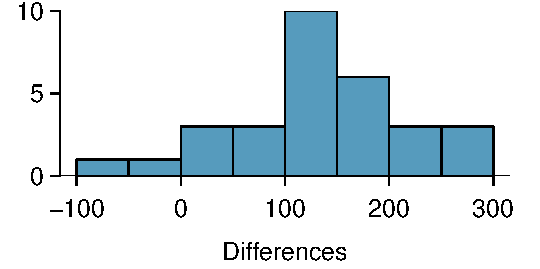
\includegraphics[width=0.45\textwidth]{ch_inference_for_means/figures/satImprovementHTDataHistogram/satImprovementHTDataHistogram}
\caption{SAT score after course - SAT score before course. }
\label{satImprovementHTDataHistogram3}
\end{figure}


\begin{exercisewrap}
\begin{nexercise}
Based on the interval (105.2, 166.6), calculated previously, can we say that 95\% of student scores increased between 105.2 and 166.6 points after taking the company's course?  

\index{data!SAT prep company|)}

\end{nexercise}
\end{exercisewrap}
\footnotetext{No.  This interval is attempting to capture the \emph{average} increase.  It is not attempting to capture 95\% of the increases.  Looking at Figure~\ref{satImprovementHTDataHistogram3}, we see that only a small percent had increases between 105.2 and 166.6.}


%%
\subsection[Calculator: the matched pairs $t$-interval]{Calculator: the matched pairs \pmb{$t$}-interval}
\label{matchedpairstint}


\begin{onebox}{TI-83/84: matched pairs T-interval}
Use \calctext{STAT}, \calctext{TESTS}, \calctext{TInterval}.
\begin{enumerate}
\setlength{\itemsep}{0mm}
\item Choose \calctext{STAT}.
\item Right arrow to \calctext{TESTS}.
\item Down arrow and choose \calctext{8:TInterval}.
\item Choose \calctext{Data} if you have all the data or \calctext{Stats} if you have the mean and standard deviation.\vspace{-1.5mm}
\begin{itemize}
\item If you choose \calctext{Data}, let \calctext{List} be \calctext{L3} or the list in which you entered the differences (don't forget to enter the differences!) and let \calctext{Freq} be \calctext{1}.
\item If you choose \calctext{Stats}, enter the mean, $SD$, and sample size of the differences.
\end{itemize}
\item Let \calctext{C-Level} be the desired confidence level.
\item Choose \calctext{Calculate} and hit \calcbutton{ENTER}, which returns: \\[1mm]
\begin{tabular}{l l}
\calctext{(\underline{\ \ },\underline{\ \ })} & the confidence interval for the mean of the differences \\
$\calctextmath{\bar{x}}$ & the sample mean of the differences \\
\calctext{Sx} & the sample $SD$ of the differences \\
\calctext{n} & the number of differences in the sample
\end{tabular}
\end{enumerate}
\end{onebox}

\begin{onebox}{Casio fx-9750GII: matched pairs T-interval}
\begin{enumerate}
\setlength{\itemsep}{0mm}
\item Compute the paired differences of the observations.
\item Using the computed differences, follow the instructions for a 1-sample $t$-interval.
\end{enumerate}
\end{onebox}

\begin{center}
\begin{tabular}{ccccc}
\hline
$n_{_{\text{\emph{diff}}}}$	&\hspace{3mm}& $\bar{x}_{_{\text{\emph{diff}}}}$	&\hspace{3mm}& $s_{_{\text{\emph{diff}}}}$ \vspace{1mm}\\
\uclabookN{}  && \uclabookM{}  && \uclabookSD{} \\
\hline
\end{tabular}
\end{center}

\begin{exercisewrap}
\begin{nexercise}
In our UCLA textbook example, we had 68 paired differences.  Because $df=67$ was not on our $t$-table, we rounded the $df$ down to 60.  This gave us a 95\% confidence interval (0.325, 6.834).  Use a calculator to find the more exact 95\% confidence interval based on 67 degrees of freedom.  How different is it from the one we calculated based on 60 degrees of freedom?\footnotemark
\end{nexercise}
\end{exercisewrap}
\footnotetext{Choose \calctext{TInterval} or equivalent.  We do not have all the data, so choose \calctext{Stats} on a TI or \calctext{Var} on a Casio.  Enter $\calctextmath{\bar{x}}$ = 3.58 and $\calctextmath{Sx}$ = 13.42.  Let $\calctext{n}=68$ and \calctext{C-Level} = 0.95.  This should give the interval $(0.332,\ 6.828$).  The intervals are equivalent when rounded to two decimal places.}


\D{\newpage}

%%
\subsection*{Section summary}

\begin{itemize} 
\item Paired data can come from a {random sample} or a {matched pairs experiment}.   With paired data, we are often interested in whether the \emph{difference} is positive, negative, or zero.  For example, the difference of paired data from a matched pairs experiment tells us whether one treatment did better, worse, or the same as the other treatment for each subject.

\item We use the notation $\bar{x}_{\text{\emph{diff}}}$ to represent the mean of the sample differences.  Likewise, $s_{\text{\emph{diff}}}$ is the standard deviation of the sample differences, and $n_{\text{\emph{diff}}}$ is the number of sample differences.


\item To carry out inference on paired data, we first find all of the sample differences.  Then, we perform a one-sample procedure on the \emph{differences}.  For this reason, the confidence interval and hypothesis test for paired data use the same $t$-procedures as the one-sample methods, where the degrees of freedom is given by $n_{\text{\emph{diff}}}-1$.


\item When there is paired data and the parameter of interest is a mean of the differences:  
\begin{itemize}
\item Estimate $\mu_{\text{\emph{diff}}}$ at the C\% confidence level using a \term{matched pairs $t$-interval}.
\item Test $H_0$: $\mu_{\text{\emph{diff}}}=0$ at the $\alpha$ significance level using a \term{matched pairs $t$-test}. 
\end{itemize}

\item The conditions for the matched pairs $t$-interval and $t$-test are the same.  
\begin{itemize}
\item[1.]  There is paired data from a random sample or a matched pairs experiment.
\item[2.]  $n_{\text{\emph{diff}}}\ge 30$ or the population of differences is nearly normal.
 \item[] If the number of differences is less than 30 and it is not known that the population of differences is nearly normal, we argue that the population of differences could be nearly normal if there is no strong skew or outliers in the sample differences.
\end{itemize}


\item When the conditions are met, we calculate the confidence interval and the test statistic as we did in the previous section.  Here, our data is a list of differences.

\begin{itemize}
\setlength{\itemsep}{2mm}
\item[] Confidence interval:\ \  $\text{point estimate}\ \pm\ t^{\star} \times SE\ \text{of estimate}$
\item[] Test statistic:  $T = \frac{\text{point estimate } - \text{ null value}}{SE \text{ of estimate}}$ 
\end{itemize}
Here the point estimate is the mean of sample differences: $\bar{x}_{\text{\emph{diff}}}$.
\item[] The $SE$ of estimate is the $SE$ of a mean of sample differences: $\frac{s_{\text{\emph{diff}}}}{\sqrt{n_{\text{\emph{diff}}}}}$.
\item[] The degrees of freedom is given by $df = n_{\text{\emph{diff}}}-1$.

\end{itemize}


%%%%%Section exercises
{\exercisesheader{}

% 15

\eoce{\qt{Air quality\label{air_quality_shortened}}
Air quality measurements were collected in 
a random sample of 25 country capitals in 2013, and then again in the same 
cities in 2014. We would like to use these data to compare
average air quality between the two years.
Should we use a paired or non-paired test? Explain your reasoning.
}{}

% 16

\eoce{\qt{True / False: paired\label{tf_paired}} Determine if the following 
statements are true or false. If false, explain.
\begin{parts}
\item In a paired analysis we first take the difference of each pair of observations, 
and then we do inference on these differences.
\item Two data sets of different sizes cannot be analyzed as paired data.
\item Consider two sets of data that are paired with each other.
Each observation in one data set has a natural correspondence with 
exactly one observation from the other data set.
\item Consider two sets of data that are paired with each other.
Each observation in one data set is subtracted from the average of the 
other data set's observations.
\end{parts}
}{}

% 17

\eoce{\qt{Paired or not? Part I\label{paired_or_not_1}} In each of the following 
scenarios, determine if the data are paired.
\begin{parts}
\item Compare pre- (beginning of semester) and post-test (end of semester) 
scores of students.
\item Assess gender-related salary gap by comparing salaries of randomly 
sampled men and women.
\item Compare artery thicknesses at the beginning of a study and after 2 years 
of taking Vitamin E for the same group of patients.
\item Assess effectiveness of a diet regimen by comparing the before and after 
weights of subjects.
\end{parts}
}{}

% 18

\eoce{\qt{Paired or not? Part II\label{paired_or_not_2}} In each of the following 
scenarios, determine if the data are paired.
\begin{parts}
\item We would like to know if Intel's stock and Southwest Airlines' stock have 
similar rates of return. To find out, we take a random sample of 50 days, and 
record Intel's and Southwest's stock on those same days.
\item We randomly sample 50 items from Target stores and note the price for 
each. Then we visit Walmart and collect the price for each of those same 50 
items.
\item A school board would like to determine whether there is a difference in 
average SAT scores for students at one high school versus another high school 
in the district. To check, they take a simple random sample of 100 students 
from each high school.
\end{parts}
}{}

% 19

\eoce{\qt{Global warming, Part I\label{global_warming_v2_1}}
Let's consider a limited set of climate data,
examining temperature differences in 1948 vs~2018.
We randomly sampled 197 locations from the
National Oceanic and Atmospheric Administration's
(NOAA) historical data,
where the data was available for both years of interest.
We want to know: were there more days with temperatures
exceeding 90\textdegree{}F in 2018 or
in~1948?\footfullcite{webpage:noaa_1948_2018}
The difference in number of days exceeding 90\textdegree{}F
(number of days in 2018 - number of days in 1948) was calculated
for each of the 197 locations.
The average of these differences was 2.9 days with 
a standard deviation of 17.2 days.
We are interested in determining whether these data provide
strong evidence that there were more days in 2018 that
exceeded 90\textdegree{}F from NOAA's weather
stations.\vspace{3mm}

\noindent%
\begin{minipage}[c]{0.65\textwidth}
\begin{parts}
\item
    Is there a relationship between the observations collected
    in 1948 and 2018?
    Or are the observations in the two groups independent?
    Explain.
\item
    Write hypotheses for this research in symbols and in words.
\item
    Check the conditions required to complete this test.
    A histogram of the differences is given to the right.
\item
    Calculate the test statistic and find the p-value.
\item
    Use $\alpha = 0.05$ to evaluate the test,
    and interpret your conclusion in context.
\item
    What type of error might we have made?
    Explain in context what the error means.
\end{parts}
\end{minipage}
\begin{minipage}[c]{0.02\textwidth}
\ 
\end{minipage}
\begin{minipage}[c]{0.32\textwidth}
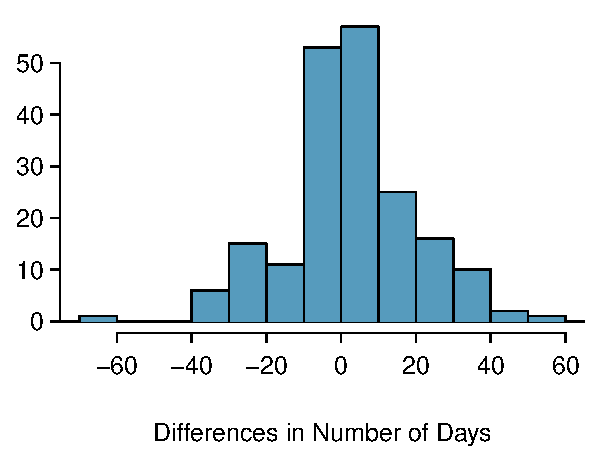
\includegraphics[width=\textwidth]{ch_inference_for_means/figures/eoce/global_warming_v2_1/global_warming_v2_1_diffs}
\end{minipage}
% library(openintro); d <- climate70$dx90_2018 - climate70$dx90_1948; mean(d); sd(d); length(d); t.test(d)
}{}

\D{\newpage}

% 20

\eoce{\qt{High School and Beyond, Part I\label{hs_beyond_1}} The National Center of 
Education Statistics conducted a survey of high school seniors, collecting test 
data on reading, writing, and several other subjects. Here we examine a simple 
random sample of 200 students from this survey. Side-by-side box plots of 
reading and writing scores as well as a histogram of the differences in scores 
are shown below.
\begin{center}
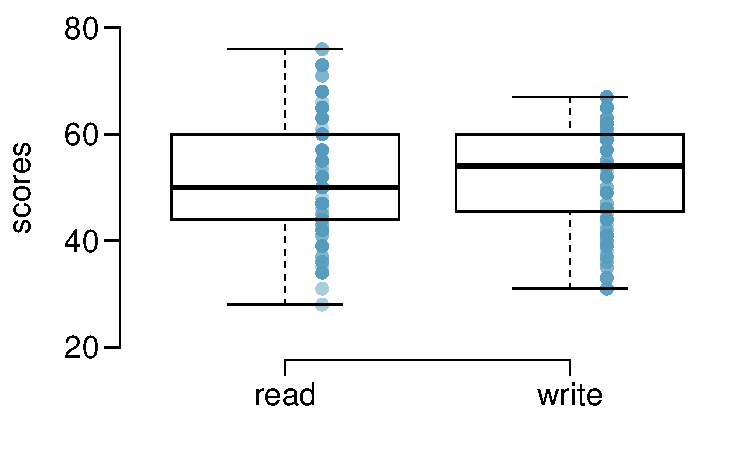
\includegraphics[width=0.44\textwidth]{ch_inference_for_means/figures/eoce/hs_beyond_1/hs_beyond_read_write_box.pdf}
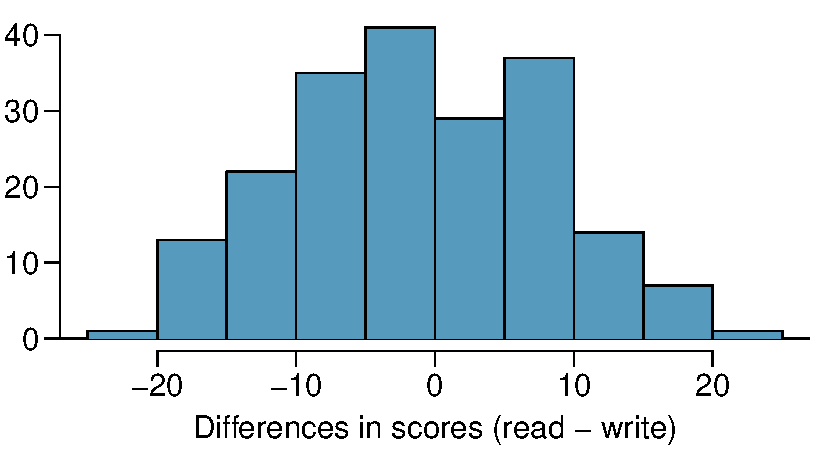
\includegraphics[width=0.54\textwidth]{ch_inference_for_means/figures/eoce/hs_beyond_1/hs_beyond_diff_hist.pdf}
\end{center}
\begin{parts}
\item Is there a clear difference in the average reading and writing scores?
\item Are the reading and writing scores of each student independent of each 
other?
\item Create hypotheses appropriate for the following research question: is 
there an evident difference in the average scores of students in the reading 
and writing exam?
% is there evidence that students on average perform differently on the reading and writing exam?
\item Check the conditions required to complete this test.
\item The average observed difference in scores is 
$\bar{x}_{read-write} = -0.545$, and the standard deviation of the differences 
is 8.887 points. Do these data provide convincing evidence of a difference 
between the average scores on the two exams?
\item What type of error might we have made? Explain what the error means in 
the context of the application.
\item Based on the results of this hypothesis test, would you expect a 
confidence interval for the average difference between the reading and writing 
scores to include 0? Explain your reasoning.
\end{parts}
}{}


% 21

\eoce{\qt{Global warming, Part II\label{global_warming_v2_2}}
We considered the change in the number of days exceeding
90\textdegree{}F from 1948 and 2018 at 197 randomly sampled
locations from the NOAA database in
Exercise~\ref{global_warming_v2_1}.
The mean and standard deviation of the reported differences
are 2.9 days and 17.2 days.
\begin{parts}
\item
    Calculate a 90\% confidence interval for the average
    difference between number of days exceeding 90\textdegree{}F
    between 1948 and 2018.
    We've already checked the conditions for you.
\item
    Interpret the interval in context.
\item
    Does the confidence interval provide convincing evidence
    that there were more days exceeding 90\textdegree{}F
    in 2018 than in 1948 at NOAA stations?
    Explain.
\end{parts}
}{}

% 22

\eoce{\qt{High school and beyond, Part II\label{hs_beyond_2}} We considered the 
differences between the reading and writing scores of a random sample of 200 
students who took the High School and Beyond Survey in Exercise~\ref{hs_beyond_1}. The 
mean and standard deviation of the differences are 
$\bar{x}_{read-write} = -0.545$ and 8.887 points.
\begin{parts}
\item Calculate a 95\% confidence interval for the average difference between 
the reading and writing scores of all students.
\item Interpret this interval in context.
\item Does the confidence interval provide convincing evidence that there is a 
real difference in the average scores? Explain.
\end{parts}
}{}
}

%________________________________
\section[Inference for the difference of two means]{Inference for the difference of two means}
\label{theTDistributionForTheDifferenceOfTwoMeans}%

\sectionintro{
\noindent%
Often times we wish to compare two groups to each other to answer questions such as the following:
\begin{itemize}
\item Does treatment using embryonic stem cells (ESCs) help improve heart function following a heart attack?
\item Is there convincing evidence that newborns from mothers who smoke have a different average birth weight than newborns from mothers who don't smoke?
\item Is there statistically significant evidence that one variation of an exam is harder than another variation?
\item Are faculty willing to pay someone named ``John" more than someone named ``Jennifer"?  If so, how much more?
\end{itemize}



%%
\subsection*{Learning objectives}
\begin{enumerate}
\setlength{\itemsep}{0mm}

\item Determine when it is appropriate to use a paired $t$-procedure versus a two-sample $t$-procedure.

\item State and verify whether or not the conditions for inference on the difference of two means using the $t$-distribution are met.

\item Be able to use a calculator or other software to find the degrees of freedom associated with a two-sample $t$-procedure.

\item Carry out a complete confidence interval procedure for the difference of two means.

\item Carry out a complete hypothesis test for the difference of two means.

\end{enumerate}
}


\D{\newpage}

%%
\subsection{Sampling distribution for the difference of two means}
\label{differenceOfTwoMeans}
Previously we explored the sampling distribution for the difference of two proportions.  Here we consider the sampling distribution for the difference of two means.  We are interested in the distribution of $\bar{x}_1-\bar{x}_2$.  We know that it is centered on $\mu_1-\mu_2$.  The standard deviation for the difference can be found as follows.

\begin{align*}
SD_{\bar{x}_{1} - \bar{x}_{2}}
    &= \sqrt{\left(SD_{\bar{x}_{1}}\right)^2 +\left(SD_{\bar{x}_{2}}\right)^2 } \\
    &= \sqrt{\left(\frac{\sigma_{1}}{\sqrt{n_1}}\right)^2 + \left(\frac{\sigma_{2}}{\sqrt{n_2}}\right)^2 } \\
	&= \sqrt{\frac{\sigma_{1}^2}{n_{1}} + \frac{\sigma_{2}^2}{n_{2}}} \\
\end{align*}

Finally, we are interested in the shape of the sampling distribution of  $\bar{x}_1-\bar{x}_2$.  It will be nearly normal when the sampling distribution of each of $\bar{x}_1$ and $\bar{x}_2$ are nearly normal.

%%%
\subsection{Checking conditions for inference on a difference of means}
When comparing two means, we carry out inference on a difference of means, $\mu_1-\mu_2$.  We will use the $t$-distribution just as we did when carrying out inference on a single mean.  The assumptions are that the observations are independent, both between groups and within groups and that the sampling distribution of $\bar{x}_1-\bar{x}_2$ is nearly normal.  We check whether these assumptions are reasonable by verifying the following conditions.
\begin{description}
\setlength{\itemsep}{0mm}
\item[Independent.] Observations can be considered independent when the data are collected from two independent random samples or, in the context of experiments, from two randomly assigned treatments.  Randomly assigning subjects to treatments is equivalent to randomly assigning treatments to subjects.  
\item[Nearly normal sampling distribution.] The sampling distribution of $\bar{x}_1-\bar{x}_2$ will be nearly normal when the sampling distribution of $\bar{x}_1$ and of $\bar{x}_2$ are nearly normal, that is when both population distributions are nearly normal or both sample sizes are at least 30.  
\end{description}

As before, if the sample sizes are small and the population distributions are not known to be nearly normal, we look at the data for excessive skew or outliers.  If we do no find excessive skew or outliers in either group, we consider the assumption that the populations are nearly normal to be reasonable.


\D{\newpage}

%%
\subsection{Confidence intervals for a difference of means}

\newcommand{\johnn}{63}
\newcommand{\jennifern}{64}
\newcommand{\johnmean}{30,238}
\newcommand{\jennifermean}{26,508}
\newcommand{\johnsd}{5567}
\newcommand{\jennifersd}{7247}
\newcommand{\johnjenniferSE}{1151}

What’s in a name?  Are employers more likely to offer interviews or higher pay to prospective employees when the name on a resume suggests the candidate is a man versus a woman?  This is a challenging question to tackle, because employers are influenced by many aspects of a resume.  Thinking back to Chapter 1 on data collection, we could imagine a host of confounding factors associated with name and gender.  How could we possibly isolate just the factor of name?  We would need an experiment in which name was the only variable and everything else was held constant.  

Researchers at Yale carried out precisely this experiment.  Their results were published in the Proceedings of the National Academy of Sciences (PNAS).\footnote{\oiRedirect{textbook-jennifer-john}{https://www.pnas.org/content/109/41/16474}} The researchers sent out resumes to faculty at academic institutions for a lab manager position.  The resumes were identical, except that on half of them the applicant’s name was John and on the other half, the applicant's name was Jennifer.  They wanted to see if faculty, specifically faculty trained in conducting scientifically objective research, held implicit gender biases.  

Unlike in the matched pairs scenario, each faculty member received only one resume.  We are interested in comparing the mean salary offered to John relative to the mean salary offered to Jennifer.  Instead of taking the average of a set of paired differences, we find the average of each group separately and take their difference.  Let
\begin{align*}
\bar{x}_1:& \text{ mean salary offered to John}\\
\bar{x}_2: &\text{ mean salary offered to Jennifer}
\end{align*}
We will use $\bar{x}_1 - \bar{x}_2$ as our point estimate for $\mu_1-\mu_2$.  The data is given in the table below.

\begin{center}
\begin{tabular}{l ccc}
\hline
Name\hspace{2mm}	& $n$	& $\bar{x}$	& $s$	\\
\hline 
John		& \johnn{}		& 		 \$\johnmean{} 	& \$\johnsd{}		 \\
Jennifer		& \jennifern{}		& \$\jennifermean{}		& \$\jennifersd{}		 \\
\hline
\end{tabular}
\end{center}
\label{summaryStatsForJohnJenniferStudy}
We can calculate the difference as 
\begin{align*}
 \bar{x}_1-\bar{x}_2 = \johnmean{} - \jennifermean{} = 3730.
\end{align*}

\begin{examplewrap}
\begin{nexample}
{Interpret the point estimate 3730.  Why might we want to construct a confidence interval?}
The average salary offered to John was \$3,730 higher than the average salary offered to Jennifer.  Because there is randomness in which faculty ended up in the John group and which faculty ended up in the Jennifer group, we want to see if the difference of \$3,730 is beyond what could be expected by random variation.  In order to answer this, we will first want to calculate the $SE$ for the difference of sample means.
\end{nexample}
\end{examplewrap}

\begin{examplewrap}
\begin{nexample}
{Calculate and interpret the $SE$ for the difference of sample means.}
\begin{align*}
SE = \sqrt{\frac{s_{1}^2}{n_{1}} + \frac{s_{2}^2}{n_{2}}} = \sqrt{\frac{(\johnsd{})^2}{\johnn{}} + \frac{(\jennifersd{})^2}{\jennifern{}}} = \johnjenniferSE{}
\end{align*}
The typical error in our estimate of $\mu_1-\mu_2$, the real difference in mean salary that the faculty would offer John versus Jennifer, is \$\johnjenniferSE{}.
\end{nexample}
\end{examplewrap}

\D{\newpage}

We see that the difference of sample means of \$3,730 is more than 3 $SE$ above 0, which makes us think that the difference being 0 is unreasonable.  We would like to construct a 95\% confidence interval for the theoretical difference in mean salary that would be offered to John versus Jennifer.  For this, we need the degrees of freedom associated with a two-sample $t$-interval.  

For the one-sample $t$-procedure, the degrees of freedom is given by the simple expression $n-1$, where $n$ is the sample size.  For the two-sample $t$-procedures, however, there is a complex formula for calculating the degrees of freedom, which is based on the two sample sizes and the two sample standard deviations.  In practice, we find the degrees of freedom using software or a calculator (see Section~\ref{2SampTint}).  If this is not possible, the alternative is to use the smaller of $n_1-1$ and $n_2-1$.

\begin{onebox}
{Degrees of freedom for two-sample T-procedures}
Use statistical software or a calculator to compute the degrees of freedom for two-sample \mbox{$t$-procedures}.  If this is not possible, use the smaller of $n_1-1$ and $n_2-1$.
\end{onebox}

\begin{examplewrap}
\begin{nexample}{Verify that conditions are met for a two-sample $t$-test.  Then, construct the 95\% confidence interval for the difference of means.}
We noted previously that this is an experiment and that the two treatments (name Jennifer and name John) were randomly assigned.  Also, both sample sizes are well over 30, so the distribution of $\bar{x}_1-\bar{x}_2$ is nearly normal.  Using a calculator, we find that $df= 114.4$.  Since 114 is not on the $t$-table, we round the degrees of freedom down to 100.\footnotemark  \ Using a $t$-table at row $df=100$ with 95\% confidence, we get a $t^{\star}$ = 1.984. We calculate the confidence interval as follows. 
\begin{align*}
\text{point estimate } &\pm \ t^{\star}\times SE \text{ of estimate}\\
3730\ &\pm \ 1.984\times \johnjenniferSE{}\\
= 3730\ &\pm \ 2284\\
= (1446&, 6014)
\end{align*}
\end{nexample}
\end{examplewrap}
\footnotetext{Using technology, we get a more precise interval, based on 114.4 $df$: (1495, 6055).}

Based on this interval, we are 95\% confident that the true difference in mean salary that these faculty would offer John versus Jennifer is between \$1,495 and \$6,055.  That is, we are 95\% confident that the mean salary these faculty would offer John for a lab manager position is between \$1,446 and \$6,014 \emph{more} than the mean salary they would offer Jennifer for the position.

The results of these studies and others like it are alarming and disturbing.\footnote{A similar study sent out identical resumes with different names to investigate the importance of perceived race.  Resumes with a name commonly perceived to be for a White person (e.g. Emily) were 50\% more likely to receive a callback than the same resume with a name commonly perceived to be for a Black person (e.g. Lakisha).  \oiRedirect{textbook-emily-lakisha}{https://www.nber.org/papers/w9873}}   One aspect that makes this bias so difficult to address is that the experiment, as well-designed as it was, cannot send us much signal about \emph{which} faculty are
discriminating.  Each faculty member received only one of the resumes.  A faculty member that offered ``Jennifer" a very low salary may have also offered ``John" a very low salary.  

We might imagine an experiment in which each faculty received both resumes, so that we could compare how much they would offer a Jennifer versus a John.  However, the matched pairs scenario is clearly not possible in this case, because what makes the experiment work is that the resumes are \emph{exactly the same} except for the name. An employer would notice something fishy if they received two identical resumes.  It is only possible to say that overall, the faculty were willing to offer John more money for the lab manager position than Jennifer.  Finding proof of bias for individual cases is a persistent challenge in enforcing anti-discrimination laws.

\D{\newpage}

\begin{onebox}{Constructing a confidence interval for the difference of two means}
To carry out a complete confidence interval procedure to estimate the difference of two means $\mu_1 - \mu_2$,
\\
\\
\inferencestep{Identify} Identify the parameter and the confidence level, C\%.
\begin{itemize}\vspace{-1mm}
\setlength{\itemsep}{0mm}
\item[] The parameter will be a difference of means, e.g. the true difference in mean cholesterol reduction (mean treatment A $-$ mean treatment B).  
\end{itemize}
 \inferencestep{Choose} Choose the appropriate interval procedure and identify it by name.  \vspace{-1mm}
\begin{itemize}
\item[] Here we choose the \term{2-sample $t$-interval}.
\end{itemize}
 \inferencestep{Check} Check conditions for the sampling distribution of $\bar{x}_1-\bar{x}_2$ to be nearly normal.\vspace{-1mm}
\begin{itemize}
\setlength{\itemsep}{0mm}
\item[] 1. Data come from 2 independent random samples or 2 randomly assigned treatments. 
\item[] 2. $n_1\ge 30$ and $n_2\ge 30$ or both population distributions are nearly normal.
\item[] \quad \ If the sample sizes are less than 30 and the population distributions are unknown, 
\item[] \quad \ check for strong skew or outliers in either data set.  If neither is found, the condition 
\item[] \quad \ that both population distributions are nearly normal is considered reasonable.  
\end{itemize}
 \inferencestep{Calculate}  Calculate the confidence interval and record it in interval form.
\begin{itemize}
\item[] $\text{point estimate}\ \pm \ t^{\star} \times SE\ \text{of estimate}$, \quad $df$: use calculator or other technology
\begin{itemize}
\item[] point estimate: the difference of sample means $\bar{x}_1 - \bar{x}_2$
\item[] $SE$ of estimate:  $\sqrt{\frac{s^2_1}{n_1}+\frac{s^2_2}{n_2}}$
\item[] $t^{\star}$: use a $t$-table at row $df$ and confidence level C\%
\end{itemize}
\item[] (\underline{\ \ \ \ \ }, \underline{\ \ \ \ \ })
\end{itemize}
 \inferencestep{Conclude} Interpret the interval and, if applicable, draw a conclusion in context.\vspace{-1mm}
\begin{itemize}
\item[] We are C\%  confident that the true \emph{difference in mean} [...] is between \underline{\ \ \ \ \ } and  \underline{\ \ \ \ \ }. If applicable, draw a conclusion based on whether the interval is entirely above, is entirely below, or contains the value 0. 
\end{itemize}\end{onebox}

\begin{examplewrap}
\begin{nexample}
{
An instructor decided to run two slight variations of the same exam. Prior to passing out the exams, she shuffled the exams together to ensure each student received a random version. Summary statistics for how students performed on these two exams are shown in Figure~\ref{summaryStatsForTwoVersionsOfExams2nd}. Anticipating complaints from students who took Version~B, she would like to evaluate whether the difference observed in the groups is so large that it provides convincing evidence that Version~B was more difficult (on average) than Version~A.  Use a 95\% confidence interval to estimate the difference in average score: version A - version B.

\begin{center}
\begin{tabular}{l rrrrr}
\hline
Version\hspace{2mm}	& $n$	& $\bar{x}$	& $s$	& min	& max  \\
\hline
A		& 30		& 79.4		& 14 	& 45		& 100 \\
B		& 30		& 74.1		& 20		& 32		& 100 \\
\hline
\end{tabular}
\end{center}
\label{summaryStatsForTwoVersionsOfExams2nd}

}
\begin{description}
\item[\inferencestep{Identify}] The parameter we want to estimate is $\mu_{1}-\mu_2$, which is the true average score under Version A $-$ the true average score under Version B.  We will estimate this parameter at the 95\% confidence level.

\item[\inferencestep{Choose}] Because we are comparing two means, we will use a 2-sample $t$-interval.

\item[\inferencestep{Check}] The data was collected from an experiment with two randomly assigned treatments, Version A and Version B of test.   Both groups sizes are 30, so the condition that they are at least 30 is met.   
\item[\inferencestep{Calculate}]  We will calculate the confidence interval as follows.
\begin{align*}
\text{point estimate}\ \pm\ t^{\star} \times SE\ \text{of estimate}
\end{align*}
The point estimate is the difference of sample means: $\bar{x}_1-\bar{x}_2 = 79.4 - 74.1 = 5.3$\\
\\
The $SE$ of a difference of sample means is:  $\sqrt{\frac{s_1^2}{n_1} + \frac{s_2^2}{n_2}} = \sqrt{\frac{14^2}{30} + \frac{20^2}{30}} = 4.46$ \\

In order to find the critical value $t^{\star}$, we must first find the degrees of freedom.  Using a calculator, we find $df=51.9$.  We round down to 50, and using a $t$-table at row $df = 50$ and confidence level 95\%, we get $t^{\star} = 2.009$.\\

The 95\% confidence interval is given by:
\begin{align*}
(79.4 - 74.1) \ \pm\  &2.009\times \sqrt{\frac{14^2}{30} + \frac{20^2}{30}}   \qquad df = 45.97\\
5.3 \ \pm\  &2.009\times 4.46 \\
=(-3&.66,\ 14.26)
\end{align*}
\item[\inferencestep{Conclude}]  We are 95\% confident that the true difference in average score between Version A and Version B is between -2.5 and 13.1 points. Because the interval contains both positive and negative values, the data do not convincingly show that one exam version is more difficult than the other, and the teacher should not be convinced that she should add points to the Version B exam scores.

\end{description}
\end{nexample}
\end{examplewrap}


\D{\newpage}

%%
\subsection[Calculator: the 2-sample $t$-interval]{Calculator: the 2-sample \pmb{$t$}-interval}
\label{2SampTint}

\begin{onebox}{\videohref{ti84_2_mean_CI} TI-83/84: 2-sample T-interval}
Use \calctext{STAT}, \calctext{TESTS}, \calctext{2-SampTInt}.
\begin{enumerate}
\setlength{\itemsep}{0mm}
\item Choose \calctext{STAT}.
\item Right arrow to \calctext{TESTS}.
\item Down arrow and choose \calctext{0:2-SampTTInt}.
\item Choose \calctext{Data} if you have all the data or \calctext{Stats} if you have the means and standard deviations.\vspace{-1.5mm}
\begin{itemize}
\setlength{\itemsep}{0mm}
\item If you choose Data, let \calctext{List1} be \calctext{L1} or the list that contains sample 1 and let \calctext{List2} be \calctext{L2} or the list that contains sample 2 (don't forget to enter the data!). Let \calctext{Freq1} and \calctext{Freq2} be \calctext{1}.
\item If you choose \calctext{Stats}, enter the mean, SD, and sample size for sample 1 and for sample 2.
\end{itemize}
\item Let \calctext{C-Level} be the desired confidence level and let \calctext{Pooled} be \calctext{No}.
\item Choose \calctext{Calculate} and hit \calcbutton{ENTER}, which returns: \\
\begin{tabular}{ll l ll}
\calctext{(\underline{\ \ },\underline{\ \ })} & the confidence interval &\quad&
	\calctext{Sx1} & SD of sample 1 \\
\calctext{df} & degrees of freedom &&
	\calctext{Sx2} & SD of sample 2 \\
$\calctextmath{\bar{x}_1}$ & mean of sample 1 &&
	\calctext{n1} & size of sample 1 \\
$\calctextmath{\bar{x}_2}$ & mean of sample 2 &&
	\calctext{n2} & size of sample 2
\end{tabular}
\end{enumerate}
\end{onebox}

\begin{onebox}{\videohref{casio_2_mean_inference} Casio fx-9750GII: 2-sample T-interval}
\begin{enumerate}
\setlength{\itemsep}{0mm}
\item Navigate to \calctext{STAT} (\calcbutton{MENU} button, then hit the \calcbutton{2} button or select \calctext{STAT}).
\item If necessary, enter the data into a list.
\item Choose the \calctext{INTR} option (\calcbutton{F4} button).
\item Choose the \calctext{t} option (\calcbutton{F2} button).
\item Choose the \calctext{2-S} option (\calcbutton{F2} button).
\item Choose either the \calctext{Var} option (\calcbutton{F2}) or enter the data in using the \calctext{List} option.
\item Specify the test details:
  \begin{itemize}
  \setlength{\itemsep}{0mm}
  \item Confidence level of interest for \calctext{C-Level}.
  \item If using the \calctext{Var} option, enter the summary statistics for each group. If using \calctext{List}, specify the lists and leave \calctext{Freq} values at \calctext{1}.
  \item Choose whether to pool the data or not.
  \end{itemize}
\item Hit the \calcbutton{EXE} button, which returns \\[1mm]
\begin{tabular}{ll}
  \calctext{Left}, \calctext{Right} & ends of the confidence interval \\
  \calctext{df} & degrees of freedom \\
  $\calctextmath{\bar{x}1}$, $\calctextmath{\bar{x}2}$ & sample means \\
  \calctext{sx1}, \calctext{sx2} & sample standard deviations \\
  \calctext{n1}, \calctext{n2} & sample sizes
\end{tabular}
\end{enumerate}
\end{onebox}

\begin{exercisewrap}
\begin{nexercise}Use the data below and a calculator to find a 95\% confidence interval for the difference in average scores between Version A and Version B of the exam from the previous example.\footnotemark
\begin{center}
\begin{tabular}{l rrrrr}
\hline
Version\hspace{2mm}	& $n$	& $\bar{x}$	& $s$	& min	& max  \\
\hline
A		& 30		& 79.4		& 14 	& 45		& 100 \\
B		& 30		& 74.1		& 20		& 32		& 100 \\
\hline
\end{tabular}
\end{center}
\end{nexercise}
\end{exercisewrap}
\footnotetext{Choose \calctext{2-SampTInt} or equivalent.  Because we have the summary statistics rather than all of the data, choose \calctext{Stats}.  Let $\calctextmath{\bar{x}1}$=79.41, $\calctextmath{Sx1}$=14, $\calctextmath{n1}$=30, $\calctextmath{\bar{x}2}$=74.1, $\calctextmath{Sx2}=20$, and $\calctextmath{n2}=30$.  The interval is $(-3.6, 14.2)$ with $df=51.9$.}



%%
\subsection{Hypothesis testing for the difference of two means}
%Do not include the test with pooled standard deviations are grouped but mention it as one method that is discussed in other books. The reason: this is a poor test. If the sd's are remotely similar then the result will be basically the same as the sd's are not assumed to be the same. It is a big assumption that can cause problems with almost no benefits.

\index{data!baby\_smoke|(}

Four cases from a data set called \data{ncbirths}, which represents mothers and their newborns in North Carolina, are shown in Figure~\ref{babySmokeDF}. We are particularly interested in two variables: \var{weight} and \var{smoke}. The \var{weight} variable represents the weights of the newborns and the \var{smoke} variable describes which mothers smoked during pregnancy. We would like to know, is there convincing evidence that newborns from mothers who smoke have a different average birth weight than newborns from mothers who don't smoke? The smoking group includes a random sample of 50 cases and the nonsmoking group contains a random sample of 100 cases, represented in Figure~\ref{babySmokePlotOfTwoGroupsToExamineSkew}.

\begin{figure}[h]
\centering
\begin{tabular}{rrrrrll}
  \hline
 & fAge & mAge & weeks & weight & sex & smoke \\ 
  \hline
1 & NA & 13 &  37 & 5.00 & female & nonsmoker \\ 
  2 & NA & 14 &  36 & 5.88 & female & nonsmoker \\ 
  3 & 19 & 15 &  41 & 8.13 & male & smoker \\ 
  $\vdots$ &   $\vdots$ &   $\vdots$ &   $\vdots$ &   $\vdots$ &   $\vdots$ \\
  150 & 45 & 50 &  36 & 9.25 & female & nonsmoker \\ 
   \hline
\end{tabular}
\caption{Four cases from the \data{ncbirths} data set. The value ``NA'', shown for the first two entries of the first variable, indicates pieces of data that are missing.}
\label{babySmokeDF}
\end{figure}

\begin{figure}[hhh]
\centering
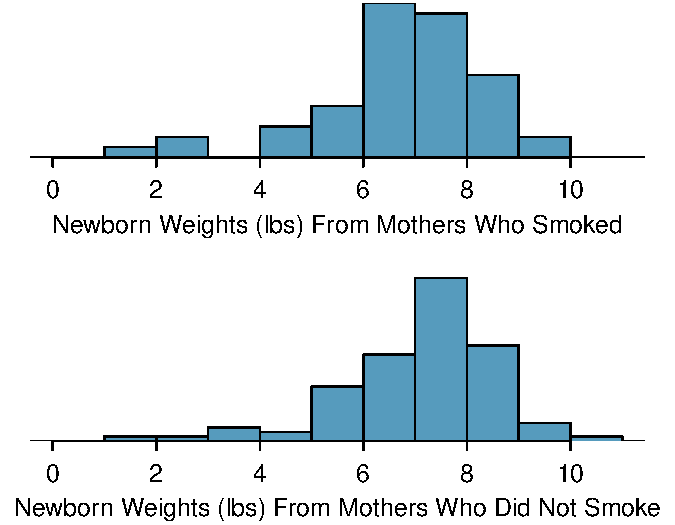
\includegraphics[width=0.63\textwidth]{ch_inference_for_means/figures/babySmokePlotOfTwoGroupsToExamineSkew/babySmokePlotOfTwoGroupsToExamineSkew}
\caption{The top panel represents birth weights for infants whose mothers smoked. The bottom panel represents the birth weights for infants whose mothers who did not smoke. The distributions exhibit moderate-to-strong and strong~skew, respectively.\index{skew!example: strong}}
\label{babySmokePlotOfTwoGroupsToExamineSkew}
\end{figure}

\D{\newpage}

\begin{examplewrap}
\begin{nexample}{Set up appropriate hypotheses to evaluate whether there is a relationship between a mother smoking and average birth weight.}\label{babySmokeHTForWeight}
Let $\mu_{1}$ represent the mean for mothers that did smoke and $\mu_2$ represent the mean for mothers that did not smoke.  We will take the difference as: smoker $-$ nonsmoker.  The null hypothesis represents the case of no difference between the groups.
\begin{itemize}
\setlength{\itemsep}{0mm}
\item[$H_0$:] $\mu_{1} - \mu_{2} = 0$.  There is no difference in average birth weight for newborns from mothers who did and did not smoke. 
\item[$H_A$:] $\mu_{1} - \mu_{2} \neq 0$. There is some difference in average newborn weights from mothers who did and did not smoke.
\end{itemize}
\end{nexample}
\end{examplewrap}

We check the two conditions necessary to use the $t$-distribution to the difference in sample means. (1)~Because the data come from a sample, we need there to be two independent random samples.  In fact, there was only one random sample, but it is reasonable that the two groups here are independent of each other, so we will consider the assumption of independence reasonable.  (2)~The sample sizes of 50 and 100 are well over 30, so we do not worry about the distributions of the original populations.  Since both conditions are satisfied, the difference in sample means may be modeled using a $t$-distribution.

%Summary statistics are shown for each sample in Figure~\ref{summaryStatsOfBirthWeightForNewbornsFromSmokingAndNonsmokingMothers}.

\begin{figure}[hhh]
\centering
\begin{tabular}{lrr}
	& \resp{smoker} & \resp{nonsmoker} \\
\hline
mean & 6.78 & 7.18 \\
st. dev. & 1.43 & 1.60 \\
samp. size & 50 & 100 \\
\hline
\end{tabular}
\caption{Summary statistics for the \data{ncbirths} data set.}
\label{summaryStatsOfBirthWeightForNewbornsFromSmokingAndNonsmokingMothers}
\end{figure}

\begin{examplewrap}
\begin{nexample}
{We will use the summary statistics in Figure~\ref{summaryStatsOfBirthWeightForNewbornsFromSmokingAndNonsmokingMothers} for this exercise.
\\ (a)~What is the point estimate of the population difference, $\mu_{1} - \mu_{2}$? 
\\(b)~Compute the standard error of the point estimate from part (a).}
(a)~The point estimate is the difference of sample means: $\bar{x}_{1} - \bar{x}_{2} = 6.78-7.18=-0.40$ pounds. \\
(b)~The standard error for a difference of sample means is calculated analogously to the standard deviation for a difference of sample means.
\begin{eqnarray*}
SE = \sqrt{\frac{s_1^2}{n_1} + \frac{s_1^2}{n_1}}
	= \sqrt{\frac{1.43^2}{100} + \frac{1.60^2}{50}}
	= 0.26 \text{ pounds}
\end{eqnarray*}
\end{nexample}
\end{examplewrap}


\begin{examplewrap}
\begin{nexample}{Compute the test statistic. } \label{babySmokeHTForWeightComputePValueAndEvalHT}
We have already found the point estimate and the $SE$ of estimate.  The null hypothesis is that the two means are equal, or that their difference equals 0.  The null value for the difference, therefore is~0.  We now have everything we need to compute the test statistic.
\begin{eqnarray*}
T = \frac{\text{point estimate} - \text{null value}}{SE \text{ of estimate}} = \frac{\ 0.40 - 0\ }{0.26} = 1.54
\end{eqnarray*}
\end{nexample}
\end{examplewrap}

\begin{examplewrap}
\begin{nexample}{Draw a picture to represent the p-value for this hypothesis test, then calculate the p-value.}
\label{pictureOfPValueForEstimateOfDiffOfMeansOfBirthWeights}
To depict the p-value, we draw the distribution of the point estimate as though $H_0$ were true and shade areas representing at least as much evidence against $H_0$ as what was observed. Both tails are shaded because it is a two-sided test.
\begin{center}
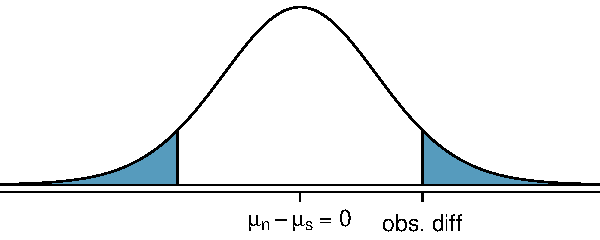
\includegraphics[width=0.6\textwidth]{ch_inference_for_means/figures/distOfDiffOfSampleMeansForBWOfBabySmokeData/distOfDiffOfSampleMeansForBWOfBabySmokeData}
\end{center}
We saw previously that the degrees of freedom can be found using software or using the smaller of $n_1-1$ and $n_2-1$.  If we use $50-1=49$ degrees of freedom, we find that the area in the upper tail is 0.065.  The p-value is twice this, or $2\times 0.065= 0.130$.  See Section~\ref{2SampTtest} for a shortcut to compute the degrees of freedom and p-value on a calculator.
\end{nexample}
\end{examplewrap}

\begin{examplewrap}
\begin{nexample}{What can we conclude from this p-value?  Use a significance level of $\alpha=0.05$.  }
\label{pictureOfPValueForEstimateOfDiffOfMeansOfBirthWeights}
This p-value of 0.130 is larger the significance level of 0.05, so we do not reject the null hypothesis. There is not sufficient evidence to say there is a difference in average birth weight of newborns from North Carolina mothers who did smoke during pregnancy and newborns from North Carolina mothers who did not smoke during pregnancy.
\end{nexample}
\end{examplewrap}




\begin{examplewrap}
\begin{nexample}
{Does the conclusion to Example~\ref{babySmokeHTForWeightComputePValueAndEvalHT} mean that smoking and average birth weight are unrelated?}
Not necessarily. It is possible that there is some difference but that we did not detect it.  The result must be considered in light of other evidence and research.  In fact, larger data sets do tend to show that women who smoke during pregnancy have smaller newborns.
\end{nexample}
\end{examplewrap}


\begin{exercisewrap}
\begin{nexercise}
If we made an error in our conclusion, which type of error could we have made: Type~I or Type~II?\footnotemark
\end{nexercise}
\end{exercisewrap}
\footnotetext{Since we did not reject $H_0$, it is possible that we made a Type~II Error.  It is possible that there is some difference but that we did not detect it. }


\begin{exercisewrap}
\begin{nexercise} \label{babySmokeHTIDingHowToDetectDifferences}
If we made a Type~II Error and there is a difference, what could we have done differently in data collection to be more likely to detect the difference?\footnotemark
\end{nexercise}
\end{exercisewrap}
\footnotetext{We could have collected more data. If the sample sizes are larger, we tend to have a better shot at finding a difference if one exists.  In other words, increasing the sample size increases the power of the test.}
% Resource on this topic:
% http://archive.tobacco.org/Documents/documentquotes.html

\index{data!baby\_smoke|)}

\D{\newpage}

\begin{onebox}{Hypothesis test for the difference of two means}
To carry out a complete hypothesis test to test the claim that two means $\mu_1$ and $\mu_2$ are equal to each other,
\\
\\
\inferencestep{Identify} Identify the hypotheses and the significance level, $\alpha$.
\begin{itemize}\vspace{-1mm}
\setlength{\itemsep}{0mm}
\item[] $H_0$: $\mu_1=\mu_2$  
\item[] $H_A$: $\mu_1\ne \mu_2$; \quad $H_A$: $\mu_1>\mu_2$; \quad or \quad $H_A$: $\mu_1<\mu_2$ 
\end{itemize}
 \inferencestep{Choose} Choose the appropriate test procedure and identify it by name. \vspace{-1mm}
\begin{itemize}
\item[] Here we choose the \term{2-sample $t$-test}.
\end{itemize}
 \inferencestep{Check} Check conditions for the sampling distribution of $\bar{x}_1-\bar{x}_2$ to be nearly normal.\vspace{-1mm}
\begin{itemize}
\setlength{\itemsep}{0mm}
\item[] 1. Data come from 2 independent random samples or 2 randomly assigned treatments. 
\item[] 2. $n_1\ge 30$ and $n_2\ge 30$ or both population distributions are nearly normal.
\item[] \quad \ If the sample sizes are less than 30 and the population distributions are unknown, 
\item[] \quad \ check for excessive skew or outliers in either data set.  If neither is found, the condition 
\item[] \quad \ that both population distributions are nearly normal is considered reasonable.  
\end{itemize}
 \inferencestep{Calculate}  Calculate the $t$-statistic, $df$, and p-value.
\begin{itemize}
\item[] $T = \frac{\text{point estimate } - \text{ null value}}{SE \text{ of estimate}}$ \quad $df$: use calculator or other technology
\begin{itemize}
\item[] point estimate: the difference of sample means $\bar{x}_1 - \bar{x}_2$
\item[] $SE$ of estimate:  $\sqrt{\frac{s^2_1}{n_1}+\frac{s^2_2}{n_2}}$
\end{itemize}
\item[] p-value = (based on the $t$-statistic, the $df$, and the direction of $H_A$)
\end{itemize}
 \inferencestep{Conclude} Compare the p-value to $\alpha$, and draw a conclusion in context.\vspace{-1mm}
\begin{itemize}
\item[] If the p-value is $< \alpha$, reject $H_0$; there is sufficient evidence that [$H_A$ in context]. 
\item[] If the p-value is $> \alpha$, do not reject $H_0$; there is not sufficient evidence that [$H_A$ in context].
\end{itemize}\end{onebox}




\D{\newpage}
\index{data!stem cells, heart function|(}

\begin{examplewrap}
\begin{nexample} 
{\label{exerciseToEvaluteWhetherESCsAreHelpfulInImprovingHeartFunctionInSheep}
Do embryonic stem cells (ESCs) help improve heart function following a heart attack? The following table and figure summarize results from an experiment to test ESCs in sheep that had a heart attack.
\begin{center}
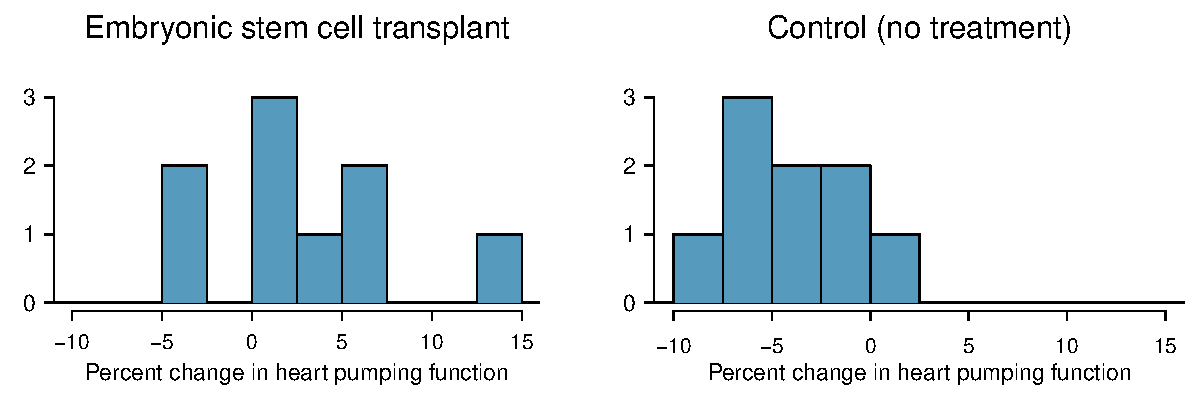
\includegraphics[width=0.95\textwidth]{ch_inference_for_means/figures/stemCellTherapyForHearts/stemCellTherapyForHearts}

\begin{tabular}{l rrrrr}
\hline
\hspace{10mm}	& $n$	& $\bar{x}$	& $s$  	 \\
\hline
ESCs		& 9		& 3.50		& 5.17  	\\
control		& 9		& -4.33		& 2.76  	 \\
\hline
\end{tabular}
\end{center}
Each of these sheep was randomly assigned to the ESC or control group, and the change in their hearts' pumping capacity was measured. A positive value generally corresponds to increased pumping capacity, which suggests a stronger recovery. The sample data is also graphed.  Use the given information and an appropriate statistical test to answer the research question.
}
\begin{description}
\item[\inferencestep{Identify}]  Let $\mu_1$ be the mean percent change for sheep that receive ESC and let $\mu_2$ be the mean percent change for sheep in the control group.  We will use an $\alpha=0.05$ significance level. \\
$H_0$: $\mu_{1} - \mu_{2} = 0$. The stem cells do not improve heart pumping function.\\
$H_A$: $\mu_{1} - \mu_{2} > 0$. The stem cells do improve heart pumping function.

\item[\inferencestep{Choose}] Because we are hypothesizing about a difference of means we choose the \mbox{2-sample $t$-test.}
\item[\inferencestep{Check}]  The data come from an experiment with two randomly assigned treatments.  The group sizes are small, but the data show no excessive skew or outliers, so the assumption that the population distributions are normal is reasonable.
\item[ \inferencestep{Calculate} ]  We will calculate the $t$-statistic and the p-value.
\begin{align*}
T = \frac{\text{point estimate } - \text{ null value}}{SE \text{ of estimate}}
\end{align*}
The point estimate is the difference of sample means: $ \bar{x}_{1} - \bar{x}_{2}=3.50 - (-4.33) = 7.83$\\
\\
The $SE$ of a difference of sample means: $\sqrt{\frac{s_1^2}{n_1} + \frac{s_2^2}{n_2}}= \sqrt{\frac{(5.17)^2}{9} + \frac{(2.76)^2}{9}} = 1.95$
\begin{align*}
T = \frac{3.50 - (-4.33) - 0}{\sqrt{\frac{(5.17)^2}{9} + \frac{(2.76)^2}{9}} } = \frac{7.83 - 0}{1.95} = 4.01 
\end{align*}
Because $H_A$ is an upper tail test ( $>$ ), the p-value corresponds to the area to the right of $t=4.01$ with the appropriate degrees of freedom.  Using a calculator, we find get $df=12.2$ and p-value $ = 8.4\times 10^{-4}=0.00084$.  
\item[\inferencestep{Conclude}]  The p-value is much less than 0.05, so we reject the null hypothesis. There is sufficient evidence that embryonic stem cells improve the heart's pumping function in sheep that have suffered a heart attack.

\end{description}

\end{nexample}
\end{examplewrap}


\D{\newpage}

%%
\subsection[Calculator: the 2-sample $t$-test]{Calculator: the 2-sample \pmb{$t$}-test}
\label{2SampTtest}

\begin{onebox}{\videohref{ti84_2_mean_HT} TI-83/84: 2-sample T-test}
Use \calctext{STAT}, \calctext{TESTS}, \calctext{2-SampTTest}.
\begin{enumerate}
\setlength{\itemsep}{0mm}
\item Choose \calctext{STAT}.
\item Right arrow to \calctext{TESTS}.
\item Choose \calctext{4:2-SampTTest}.
\item Choose \calctext{Data} if you have all the data or \calctext{Stats} if you have the means and standard deviations.\vspace{-1.5mm}
\begin{itemize}
\setlength{\itemsep}{0mm}
\item If you choose \calctext{Data}, let \calctext{List1} be \calctext{L1} or the list that contains sample 1 and let \calctext{List2} be \calctext{L2} or the list that contains sample 2 (don't forget to enter the data!). Let \calctext{Freq1} and \calctext{Freq2} be \calctext{1}.
\item If you choose \calctext{Stats}, enter the mean, SD, and sample size for sample 1 and for sample 2
\end{itemize}
\item Choose $\calctextmath{\ne}$, $\calctextmath{<}$, or $\calctextmath{>}$ to correspond to $H_A$.
\item Let \calctext{Pooled} be \calctext{NO}.
\item Choose \calctext{Calculate} and hit \calcbutton{ENTER}, which returns: \\[1mm]
\begin{tabular}{ll l ll}
\calctext{t} & t statistic &\quad&
	\calctext{Sx1} & SD of sample 1 \\
\calctext{p} & p-value &&
	\calctext{Sx2} & SD of sample 2 \\
\calctext{df} & degrees of freedom &&
	\calctext{n1} & size of sample 1 \\
$\calctextmath{\bar{x}_1}$ & mean of sample 1 &&
	n2 & size of sample 2 \\
$\calctextmath{\bar{x}_2}$ & mean of sample 2
\end{tabular}
\end{enumerate}
\end{onebox}

\begin{onebox}{\videohref{casio_2_mean_inference} Casio fx-9750GII: 2-sample T-test}
\begin{enumerate}
\setlength{\itemsep}{0mm}
\item Navigate to \calctext{STAT} (\calcbutton{MENU} button, then hit the \calcbutton{2} button or select \calctext{STAT}).
\item If necessary, enter the data into a list.
\item Choose the \calctext{TEST} option (\calcbutton{F3} button).
\item Choose the \calctext{t} option (\calcbutton{F2} button).
\item Choose the \calctext{2-S} option (\calcbutton{F2} button).
\item Choose either the \calctext{Var} option (\calcbutton{F2}) or enter the data in using the \calctext{List} option.
\item Specify the test details:
  \begin{itemize}
  \setlength{\itemsep}{0mm}
  \item Specify the sidedness of the test using the \calcbutton{F1}, \calcbutton{F2}, and \calcbutton{F3} keys.
  \item If using the \calctext{Var} option, enter the summary statistics for each group. If using \calctext{List}, specify the lists and leave \calctext{Freq} values at \calctext{1}.
  \item Choose whether to pool the data or not.
  \end{itemize}
\item Hit the \calcbutton{EXE} button, which returns \\[1mm]
\begin{tabular}{ll l ll}
$\calctextmath{\mu1}\ \_\_\ \calctextmath{\mu2}$ & alt. hypothesis &&
	$\calctextmath{\bar{x}1}$, $\calctextmath{\bar{x}2}$ & sample means \\
\calctext{t} & t statistic &&
	\calctext{sx1}, \calctext{sx2} & sample standard deviations \\
\calctext{p} & p-value &&
	\calctext{n1}, \calctext{n2} & sample sizes \\
\calctext{df} & degrees of freedom
\end{tabular}
\end{enumerate}
\end{onebox}



\begin{exercisewrap}
\begin{nexercise}
Use the data below and a calculator to find the test statistics and p-value for a one-sided test, testing whether there is evidence that embryonic stem cells (ESCs) help improve heart function for sheep that have experienced a heart attack.\footnotemark
\begin{center}
\begin{tabular}{l rrrrr}
\hline
\hspace{10mm}	& $n$	& $\bar{x}$	& $s$  	 \\
\hline
ESCs		& 9		& 3.50		& 5.17  	\\
control		& 9		& -4.33		& 2.76  	 \\
\hline
\end{tabular}
\end{center}
\end{nexercise}
\end{exercisewrap}
\footnotetext{Choose \calctext{2-SampTTest} or equivalent.  Because we have the summary statistics rather than all of the data, choose \calctext{Stats}.  Let $\calctextmath{\bar{x}1}$=3.50, $\calctextmath{Sx1}$=5.17, $\calctextmath{n1}$=9, $\calctextmath{\bar{x}2}$=-4.33, $\calctextmath{Sx2}=2.76$, and $\calctextmath{n2}=9$.  We get $\calctextmath{t}=4.01$, and the p-value $\calctext{p} = 8.4\times 10^-4=0.00084$.  The degrees of freedom for the test is $\calctext{df}=12.2$.}





\D{\newpage}

%%
\subsection*{Section summary}
\begin{itemize} 
\item This section introduced inference for a difference of means, which is distinct from inference for a mean of differences.  To calculate a difference of means, $\bar{x}_1-\bar{x}_2$, we first calculate the mean of each group, then we take the difference between those two numbers.  To calculate a mean of difference, $\bar{x}_{\text{\emph{diff}}}$, we first calculate all of the differences, then we find the mean of those differences.  
\item Inference for a difference of means is based on the $t$-distribution.  The degrees of freedom is complicated to calculate and we rely on a calculator or other software to calculate this.\footnote{If this is not available, one can use $df=min(n_1-1, n_2-1)$.}

\item When there are two samples or treatments and the parameter of interest is a difference of means:  
\begin{itemize}\vspace{-1mm}
\setlength{\itemsep}{0mm}
\item Estimate $\mu_1-\mu_2$ at the C\% confidence level using a \term{2-sample t-interval}.
\item Test $H_0$: $\mu_1-\mu_2=0$ (i.e. $\mu_1=\mu_2$) at the $\alpha$ significance level using a \term{2-sample t-test} .
\end{itemize}

\item The conditions for the two sample $t$-interval and $t$-test are the same.  
\begin{itemize}
\item[1.] The data come from 2 independent random samples or 2 randomly assigned treatments.
\item[2.] $n_1\ge 30$ and $n_2\ge 30$ or both population distributions are nearly normal.
\item[]  If the sample sizes are less than 30 and it is not known that both population distributions are nearly normal, check for excessive skew or outliers in the data.  If neither exists, the condition that both population distributions could be nearly normal is considered reasonable.
\end{itemize}



\item When the conditions are met, we calculate the confidence interval and the test statistic as follows.  

\begin{itemize}
\setlength{\itemsep}{2mm}
\item[] Confidence interval:\ \  $\text{point estimate}\ \pm\ t^{\star} \times SE\ \text{of estimate}$
\item[] Test statistic:  $T = \frac{\text{point estimate } - \text{ null value}}{SE \text{ of estimate}}$ 
\end{itemize}
Here the point estimate is the difference of sample means: $\bar{x}_1-\bar{x}_2$.
\item[] The $SE$ of estimate is the $SE$ of a difference of sample means:  $\sqrt{\frac{s^2_1}{n_1}+\frac{s^2_2}{n_2}}$.
\item[] Find and record the $df$ using a calculator or other software.

\end{itemize}

%%%%%Section exercises
{\exercisesheader{}

% 23

\eoce{\qt{Friday the 13$^{\text{th}}$, Part I\label{friday_13th_traffic}} In the 
early 1990's, researchers in the UK collected data on traffic flow, number of 
shoppers, and traffic accident related emergency room admissions on Friday the 
13$^{\text{th}}$ and the previous Friday, Friday the 6$^{\text{th}}$. The 
histograms below show the distribution of number of cars passing by a specific 
intersection on Friday the 6$^{\text{th}}$ and Friday the 13$^{\text{th}}$ for 
many such date pairs. Also given are some sample statistics, where the 
difference is the number of cars on the 6th minus the number of cars on the 13th.\footfullcite{Scanlon:1993}
\begin{center}
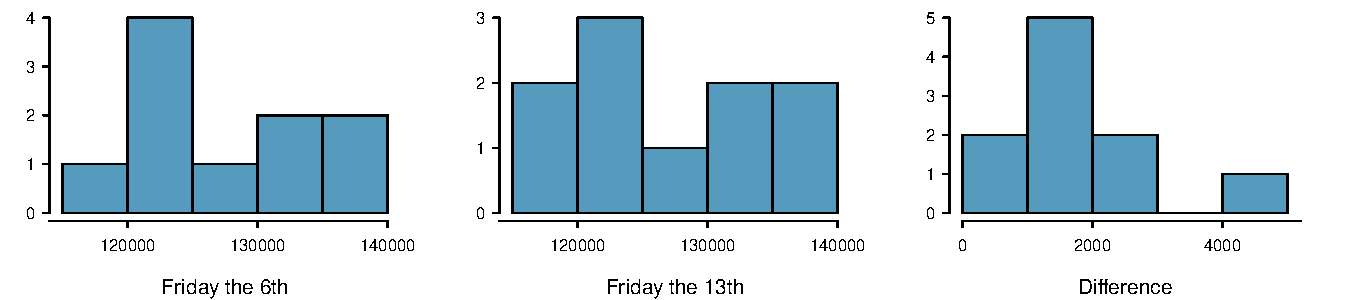
\includegraphics[width=\textwidth]{ch_inference_for_means/figures/eoce/friday_13th_traffic/friday_13th_traffic_hist} \\
$\:$ \\
{\small
\begin{tabular}{l c c c}
\hline
        & 6$^{\text{th}}$   & 13$^{\text{th}}$  & Diff.\\
\hline  
$\bar{x}$   &128,385            & 126,550       & 1,835 \\
$s$     &7,259          & 7,664         & 1,176 \\
$n$     &10             & 10                & 10 \\
\hline
\end{tabular}
}
\end{center}
\begin{parts}
\item Are there any underlying structures in these data that should be 
considered in an analysis? Explain.
\item What are the hypotheses for evaluating whether the number of people out 
on Friday the 6$^{\text{th}}$ is different than the number out on Friday the 
13$^{\text{th}}$?
\item Check conditions to carry out the hypothesis test from part~(b).
\item Calculate the test statistic and the p-value.
\item What is the conclusion of the hypothesis test?
\item Interpret the p-value in this context.
\item What type of error might have been made in the conclusion of your test? 
Explain.
\end{parts}
}{}


% 24

\eoce{\qt{Diamonds, Part I\label{diamonds_1}} Prices of diamonds are determined by 
what is known as the 4 Cs: cut, clarity, color, and carat weight. The prices of 
diamonds go up as the carat weight increases, but the increase is not smooth. 
For example, the difference between the size of a 0.99 carat diamond and a 1 
carat diamond is undetectable to the naked human eye, but the price of a 1 
carat diamond tends to be much higher than the price of a 0.99 diamond. In this 
question we use two random samples of diamonds, 0.99 carats and 1 carat, each 
sample of size 23, and compare the average prices of the diamonds. In order to 
be able to compare equivalent units, we first divide the price for each diamond 
by 100 times its weight in carats. That is, for a 0.99 carat diamond, we divide 
the price by 99. For a 1 carat diamond, we divide the price by 100. The 
distributions and some sample statistics are shown below.\footfullcite{ggplot2} \\[1mm]
\begin{minipage}[c]{0.6\textwidth}
Conduct a hypothesis test to evaluate if there is a difference between the 
average standardized prices of 0.99 and 1 carat diamonds. Make sure to state 
your hypotheses clearly, check relevant conditions, and interpret your results 
in context of the data. \\[2mm]
\begin{tabular}{l c c }
\hline
        & 0.99 carats       & 1 carat\\
\hline  
Mean    & \$44.51          & \$56.81           \\
SD      & \$13.32          &\$16.13            \\
n       &23             & 23 \\
\hline
\end{tabular}
\end{minipage}%
\begin{minipage}[c]{0.4\textwidth}
\begin{center}
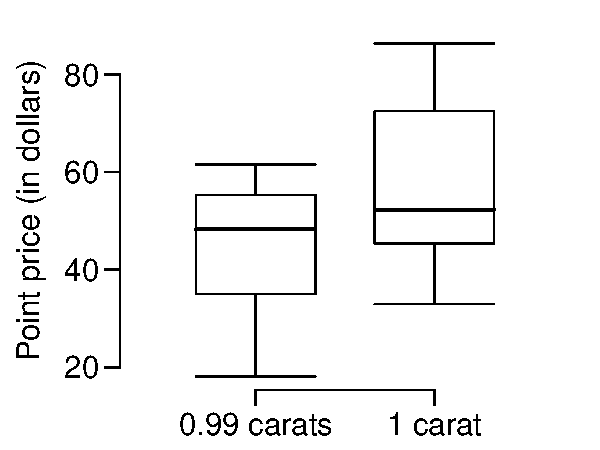
\includegraphics[width=0.85\textwidth]{ch_inference_for_means/figures/eoce/diamonds_1/diamonds_box.pdf}
\end{center}
\end{minipage}
}{}

\D{\newpage}

% 25

\eoce{\qt{Friday the 13$^{\text{th}}$, Part II\label{friday_13th_accident}}
The Friday the $13^{th}$ study reported in
Exercise~\ref{friday_13th_traffic} also provides data on traffic
accident related emergency room admissions.
The distributions of these counts from Friday the 6$^{\text{th}}$ and
Friday the 13$^{\text{th}}$ are shown below for six such paired dates
along with summary statistics.
You may assume that conditions for inference are met.
\begin{center}
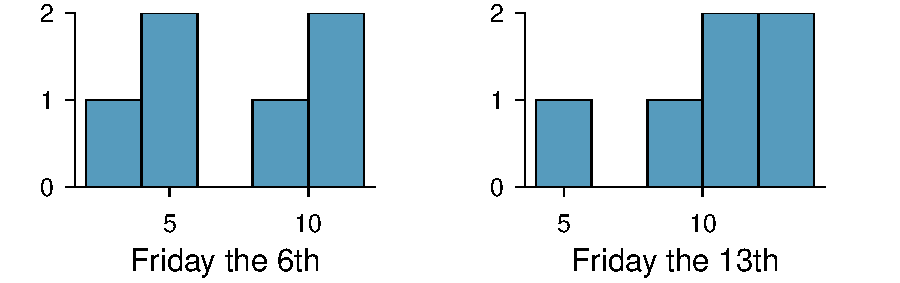
\includegraphics[width=0.74\textwidth]{ch_inference_for_means/figures/eoce/friday_13th_accident/friday_13th_accident_hist} \\
$\:$ \\
\begin{minipage}[c]{0.36\textwidth}
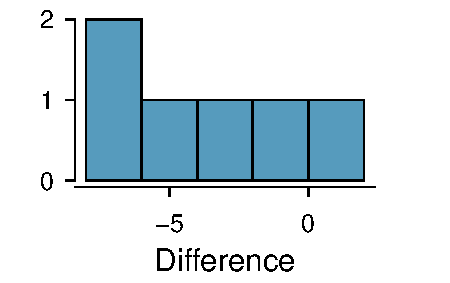
\includegraphics[width=\textwidth]{ch_inference_for_means/figures/eoce/friday_13th_accident/friday_13th_accident_hist_diff}
\end{minipage}
\begin{minipage}[c]{0.36\textwidth}
\ \ \begin{tabular}{l c c c}
\hline
        & 6$^{\text{th}}$   & 13$^{\text{th}}$  & diff\\
\hline  
Mean    &7.5                & 10.83             & -3.33 \\
SD      &3.33           & 3.6               & 3.01 \\
n       &6              & 6             & 6 \\
\hline
\end{tabular}
\end{minipage}
\end{center}

\begin{parts}
\item Conduct a hypothesis test to evaluate if there is a difference between 
the average numbers of traffic accident related emergency room admissions 
between Friday the 6$^{\text{th}}$ and Friday the~13$^{\text{th}}$.
\item Calculate a 95\% confidence interval for the difference between the 
average numbers of traffic accident related emergency room admissions between 
Friday the 6$^{\text{th}}$ and Friday the 13$^{\text{th}}$.
\item The conclusion of the original study states, ``Friday 13th is unlucky for 
some. The risk of hospital admission as a result of a transport accident may be 
increased by as much as 52\%. Staying at home is recommended.'' Do you agree 
with this statement? Explain your reasoning.
\end{parts}
}{}

% 26

\eoce{\qt{Diamonds, Part II\label{diamonds_2}} In Exercise~\ref{diamonds_1}, we 
discussed diamond prices (standardized by weight) for diamonds with weights 0.
99 carats and 1 carat. See the table for summary statistics, and then construct 
a 95\% confidence interval for the average difference between the standardized 
prices of 0.99 and 1 carat diamonds. You may assume the conditions for 
inference are met.
\begin{center}
\begin{tabular}{l c c }
\hline
        & 0.99 carats       & 1 carat\\
\hline  
Mean    & \$44.51          & \$56.81           \\
SD      & \$13.32          &\$16.13            \\
n       &23             & 23 \\
\hline
\end{tabular}
\end{center}
}{}

\D{\newpage}

% 27

\eoce{\qt{Chicken diet and weight,
    Part I\label{chick_wts_linseed_horsebean}} \videohref{ahss_eoce_sol-chick_wts_linseed_horsebean}\ \ 
Chicken farming is a multi-billion dollar industry,
and any methods that increase the growth rate of young
chicks can reduce consumer costs while increasing
company profits, possibly by millions of dollars.
An experiment was conducted to measure and compare
the effectiveness of various feed supplements on the
growth rate of chickens.
Newly hatched chicks were randomly allocated into six groups, 
and each group was given a different feed supplement.
Below are some summary statistics from this data set along
with box plots showing the distribution of weights by
feed type.\footfullcite{data:chickwts}

\noindent\begin{minipage}[c]{0.65\textwidth}
\begin{center}
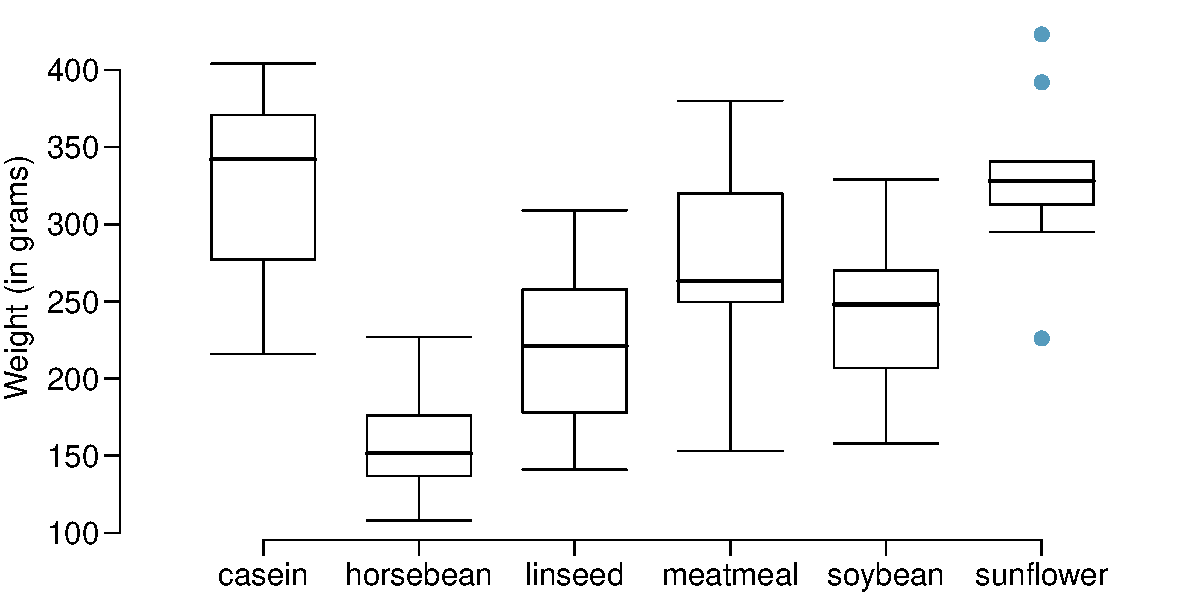
\includegraphics[width= \textwidth]{ch_inference_for_means/figures/eoce/chick_wts_linseed_horsebean/chick_wts_box.pdf}
\end{center}
\end{minipage}
\begin{minipage}[c]{0.35\textwidth}
{\footnotesize\begin{tabular}{l c c c}
\hline
            & Mean      & SD        & n \\
\hline
casein          & 323.58        & 64.43 & 12 \\
horsebean   & 160.20        & 38.63 & 10 \\
linseed         & 218.75        & 52.24 & 12 \\
meatmeal    & 276.91        & 64.90 & 11 \\
soybean         & 246.43        & 54.13 & 14 \\
sunflower       & 328.92        & 48.84 & 12 \\
\hline
\end{tabular}}
\end{minipage} 

\begin{parts}
\item Describe the distributions of weights of chickens that were fed linseed 
and horsebean.
\item Do these data provide strong evidence that the average weights of 
chickens that were fed linseed and horsebean are different? Use a 5\% 
significance level.
\item What type of error might we have committed? Explain.
\item Would your conclusion change if we used $\alpha = 0.01$?
\end{parts}
}{}

% 28

\eoce{\qt{Fuel efficiency of manual and automatic cars, Part I\label{fuel_eff_city}} 
Each year the US Environmental Protection Agency (EPA)
releases fuel economy data on cars manufactured in that year.
Below are summary statistics on fuel efficiency (in miles/gallon)
from random samples of cars with manual and automatic transmissions.
Do these data provide strong evidence of a difference between the
average fuel efficiency of cars with manual and automatic
transmissions in terms of their average city mileage?
Assume that conditions for inference are
satisfied. \footfullcite{data:epaMPG}

\noindent\begin{minipage}[c]{0.38\textwidth}
\begin{center}
\begin{tabular}{l c c }
\hline
        & \multicolumn{2}{c}{City MPG} \\
\hline
        & Automatic     & Manual         \\
Mean    & 16.12         & 19.85      \\
SD      & 3.58          & 4.51       \\
n       & 26            & 26 \\
\hline
& \\
& \\
\end{tabular}
\end{center}
\end{minipage}
\begin{minipage}[c]{0.6\textwidth}
\begin{center}
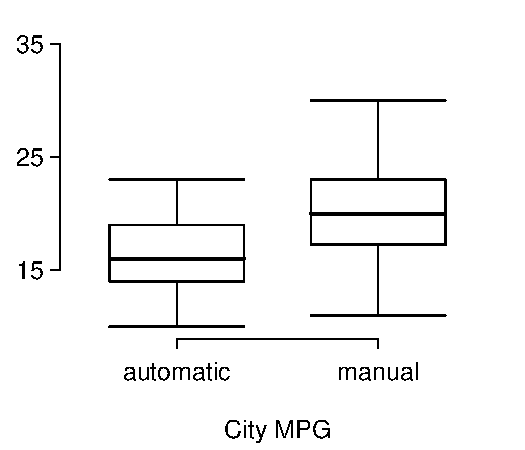
\includegraphics[width=0.7\textwidth]{ch_inference_for_means/figures/eoce/fuel_eff_city/fuel_eff_city_box.pdf}
\end{center}
\end{minipage}
}{}

% 29

\eoce{\qt{Chicken diet and weight, Part II\label{chick_wts_casein_soybean}} Casein is 
a common weight gain supplement for humans. Does it have an effect on chickens? 
Using data provided in Exercise~\ref{chick_wts_linseed_horsebean}, test the 
hypothesis that the average weight of chickens that were fed casein is 
different than the average weight of chickens that were fed soybean. If your 
hypothesis test yields a statistically significant result, discuss whether or 
not the higher average weight of chickens can be attributed to the casein diet. 
Assume that conditions for inference are satisfied.
}{}

\D{\newpage}

% 30

\eoce{\qt{Fuel efficiency of manual and automatic cars, Part II\label{fuel_eff_hway}} 
The table provides summary statistics on highway fuel economy
of the same 52 cars from Exercise~\ref{fuel_eff_city}.
Use these statistics to calculate a 98\% confidence interval
for the difference between average highway mileage of manual
and automatic cars, and interpret this interval in the context
of the data.\footfullcite{data:epaMPG}

\noindent\begin{minipage}[c]{0.38\textwidth}
\begin{center}
\begin{tabular}{l c c }
\hline
        & \multicolumn{2}{c}{Hwy MPG} \\
\hline
            & Automatic     & Manual         \\
Mean    & 22.92         & 27.88          \\
SD      & 5.29          & 5.01           \\
n       & 26            & 26 \\
\hline
& \\
& \\
\end{tabular}
\end{center}
\end{minipage}
\begin{minipage}[c]{0.6\textwidth}
\begin{center}
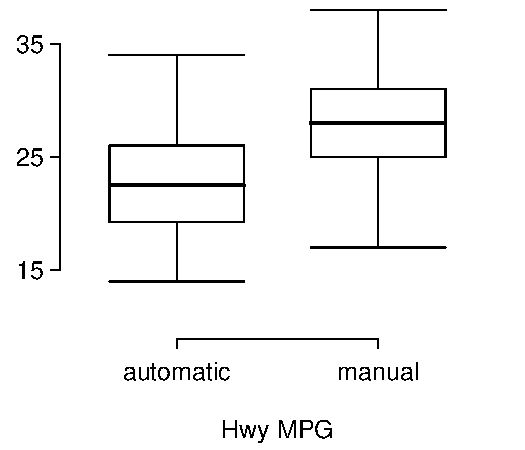
\includegraphics[width=0.7\textwidth]{ch_inference_for_means/figures/eoce/fuel_eff_hway/fuel_eff_hway_box.pdf}
\end{center}
\end{minipage}
}{}

% 31

\eoce{\qt{Prison isolation experiment, Part I\label{prison_isolation_T}}
Subjects from Central Prison in Raleigh, NC, volunteered
for an experiment involving an ``isolation'' experience.
The goal of the experiment was to find a treatment 
that reduces subjects' psychopathic deviant T scores.
This score measures a person's need for control or their rebellion against 
control, and it is part of a commonly used mental health test called the 
Minnesota Multiphasic Personality Inventory (MMPI) test. The experiment had 
three treatment groups: 
\begin{enumerate}[(1)]
\setlength{\itemsep}{0mm}
\item
    Four hours of sensory restriction plus a 15 minute
    ``therapeutic" tape advising that professional help
    is available.
\item
    Four hours of sensory restriction plus a 15 minute
    ``emotionally neutral'' tape on training hunting dogs.
\item
    Four hours of  sensory restriction but no taped message.
\end{enumerate}
Forty-two subjects were randomly assigned to these treatment groups, and an 
MMPI test was administered before and after the treatment. Distributions of the 
differences between pre and post treatment scores (pre - post) are shown below, 
along with some sample statistics. Use this information to independently test 
the effectiveness of each treatment. Make sure to clearly state your 
hypotheses, check conditions, and interpret results in the context of the data.\footfullcite{data:prison}

\begin{center}
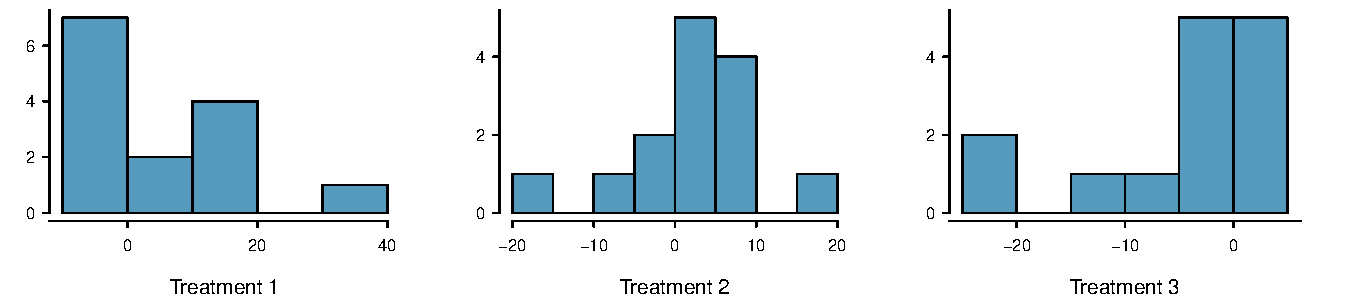
\includegraphics[width=\textwidth]{ch_inference_for_means/figures/eoce/prison_isolation_T/prison_isolation_hist} \\
$\:$ \\
\begin{tabular}{l  r  r  r  r  }
\hline
                & Tr 1  & Tr 2  & Tr 3      \\
\hline
Mean            & 6.21  & 2.86  & -3.21           \\
SD              & 12.3  & 7.94  & 8.57       \\
n               & 14        & 14        & 14     \\
\hline
\end{tabular}
\end{center}
}{}

% 32

\eoce{\qt{True / False: comparing means\label{tf_compare_means}} Determine if the 
following statements are true or false, and explain your reasoning for 
statements you identify as false.
\begin{parts}
\item When comparing means of two samples where $n_1 = 20$ and $n_2 = 40$, we 
can use the normal model for the difference in means since $n_2 \ge 30$.
\item As the degrees of freedom increases, the $t$-distribution approaches 
normality.
\item We use a pooled standard error for calculating the standard error of the 
difference between means when sample sizes of groups are equal to each other.
\end{parts}
}{}
}

%______________________________________________
\reviewchapterheader{}

\noindent We've reviewed a wide set of inference procedures over the last 3 chapters. Let's revisit each and discuss the similarities and differences among them.  The following confidence intervals and tests are structurally the same -- they all involve inference on a population parameter, where that parameter is a proportion, a difference of proportions, a mean, a mean of differences, or a difference of means. \vspace{-1mm}
\begin{itemize}
\setlength{\itemsep}{0mm}
\item 1-proportion $z$-test/interval
\item 2-proportion $z$-test/interval
\item 1-sample $t$-test/interval
\item matched pairs $t$-test/interval
\item 2-sample $t$-test/interval 
\end{itemize}
The above inferential procedures all involve a \term{point estimate}, a \term{standard error} of the estimate, and an assumption about the \term{shape of the sampling distribution} of the point estimate.
\\
\\
From Chapter~\ref{inferenceForCategoricalData}, the $\chi^2$ tests and their uses are as follows:\vspace{-1mm}
\begin{itemize}
\setlength{\itemsep}{0mm}
\item $\chi^2$ goodness of fit - compares a categorical variable to a known/fixed distribution.
\item $\chi^2$ test of homogeneity - compares a categorical variable across multiple groups.
\item $\chi^2$ test of independence - looks for association between two categorical variables. 
\end{itemize}
$\chi^2$ is a measure of \emph{overall} deviation between observed values and expected values.  These tests stand apart from the others because when using $\chi^2$ there is not a parameter of interest.  For this reason there are no confidence intervals using $\chi^2$.  Also, for $\chi^2$ tests, the hypotheses are usually written in words, because they are about the \emph{distribution} of one or more categorical variables, not about a single parameter.  
\\
\\
While formulas and conditions vary, all of these procedures follow the same basic logic and process.
\begin{itemize}\vspace{-1mm}
\setlength{\itemsep}{0mm}
\item For a confidence interval, identify the parameter to be estimated and the confidence level.  For a hypothesis test, identify the hypotheses to be tested and the significance level.
\item Choose the correct procedure.
\item Check that both conditions for its use are met.
\item Calculate the confidence interval or the test statistic and p-value, as well as the $df$ if applicable.
\item Interpret the results and draw a conclusion based on the data.
\end{itemize}
For a summary of these hypothesis test and confidence interval procedures (including one more that we will encounter in Section~\ref{inferenceForLinearRegression}), see the Inference Guide in Appendix~\ref{inferenceGuide}.



